%
% Copyright 2018 Joel Feldman, Andrew Rechnitzer and Elyse Yeager.
% This work is licensed under a Creative Commons Attribution-NonCommercial-ShareAlike 4.0 International License.
% https://creativecommons.org/licenses/by-nc-sa/4.0/
%
\questionheader{ex:s3.6.6}

%%%%%%%%%%%%%%%%%%
\subsection*{\Procedural}
%%%%%%%%%%%%%%%%%%

\begin{Mquestion}[2007H]
 Let $f(x) = x\sqrt{3 - x}$.
\begin{enumerate}[(a)]
\item\label{s3.62007_1} Find the domain of $f(x)$.
\item\label{s3.62007_2} Determine the $x$-coordinates of the local
maxima and minima (if any) and intervals where $f(x)$ is increasing or decreasing.
\item\label{s3.62007_3}  Determine intervals where $f(x)$ is concave
upwards or downwards, and the $x$ coordinates of inflection points (if any).
You may use, without verifying it, the formula $f''(x) = (3x -12)(3 - x)^{-3/2}/4$.
\item\label{s3.62007_4}  There is a point at which the tangent line to the
curve $y = f(x)$ is vertical. Find this point.
\item\label{s3.62007_6} Sketch the graph $y = f(x)$, showing
the features given in items (a) to (d) above and giving the $(x, y)$ coordinates
for all points occurring above.
\end{enumerate}
\end{Mquestion}
\begin{hint}
You'll find the intervals of increase and decrease. These will give you a basic outline of the behaviour of the function. Use  concavity to refine your picture.
\end{hint}
\begin{answer}
\eqref{s3.62007_1} $(-\infty,3]$
\\
\eqref{s3.62007_2} $f(x)$ in increasing on $(-\infty,2)$ and decreasing on $(2,3)$. There is a local maximum at $x=2$.
\\
\eqref{s3.62007_3} $f(x)$ is always concave down and has no inflection points.
\\
\eqref{s3.62007_4} $(3,0)$
\\
\eqref{s3.62007_6}
\begin{center}\begin{tikzpicture}
\YEaaxis{3}{6.4}{3}{3}
\draw plot[domain=-1.5:3, samples=100](2*\x,{\x*sqrt(3-\x)});
\draw (6,0) node[vertex, label=below:{$(3,0)$}]{};
\draw (4,2) node[vertex, label=above:{$(2.2)$}]{};
\end{tikzpicture}
\end{center}

\end{answer}
\begin{solution}
 \eqref{s3.62007_1} Since we must have $3-x \ge 0$, this tells us $x \leq 3$.
 So, the domain is $(-\infty,3]$.


\eqref{s3.62007_2}  \[f'(x)=\sqrt{3-x}-\frac{x}{2\sqrt{3-x}}
                       =3\frac{2-x}{2\sqrt{3-x}}\]
For every $x$ in the domain of $f'(x)$, the denominator is positive, so the sign of $f'(x)$ depends only on the numerator.

\begin{center}
 \begin{tabular}{|c||c|c|c|c|}
\hline
$x$  & $(-\infty,2)$ &$2$ & $(2,3)$ & $3$ \\
\hline
$f'(x)$  & positive  & 0 & negative & DNE  \\
\hline
$f(x)$ & increasing & maximum & decreasing & endpoint \\
\hline
 \end{tabular}
\end{center}

So, $f$ is increasing for $x<2$, has a local (in fact global) maximum at $x=2$,
and is decreasing for $2<x<3$.

Remark: this shows us the basic skeleton of the graph. It consists of a single hump.
\begin{center}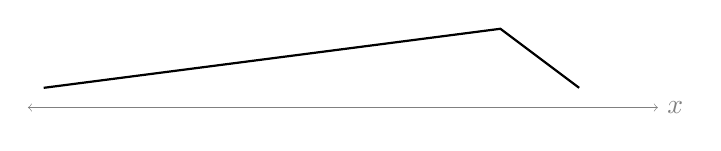
\begin{tikzpicture}
\draw[<->, help lines] (-4,0)--(4,0) node[right]{$x$};
\foreach\x in {2,3}{\YExcoord{\x}{\x}}
\draw[thick] (-3.8,.25)--(2,1)--(3,.25);
\end{tikzpicture}\end{center}

\eqref{s3.62007_3} When $x<3$,
 \[f''(x) = \frac{1}{4}(3x -12)(3 - x)^{-3/2}<0\]
The domain of $f''(x)$ is $(-\infty,-3)$, and over its domain it is always negative
 (the factor
              $(3x-12)$ is negative for all $x<4$ and the factor
              $(3-x)^{-3/2}$ is positive for all $x<3$). So, $f(x)$ has no inflection points and is concave
down everywhere.

\eqref{s3.62007_4} We already found
\begin{align*}f'(x)&=3\dfrac{2-x}{2\sqrt{3-x}}.
\intertext{ This is undefined at $x=3$. Indeed,}
\ds\lim_{x \rightarrow 3^-} 3\dfrac{2-x}{2\sqrt{3-x}}&=-\infty,
\end{align*} so
 $f(x)$ has a vertical tangent line at $(3,0)$.

\eqref{s3.62007_6}
To sketch the curve $y=f(x)$, we already know its intervals of increase and decrease, and its concavity. We also note its intercepts are $(0,0)$ and $(3,0)$.
%\centerline{\figput{OE07D_2}}
\begin{center}\begin{tikzpicture}
\YEaaxis{3}{6.4}{3}{3}
\draw plot[domain=-1.5:3, samples=100](2*\x,{\x*sqrt(3-\x)});
\draw (6,0) node[vertex, label=below:{$(3,0)$}]{};
\draw (4,2) node[vertex, label=above:{$(2.2)$}]{};
\draw[decorate, decoration={brace, amplitude=10pt, mirror}, red] (-3,-3.25)--(4,-3.25) ;
\draw[red] (.5,-4) node{increasing};
\draw[decorate, decoration={brace, amplitude=10pt, mirror}, blue] (4,-3.25)--(6,-3.25) ;
\draw[blue] (5,-4) node{decreasing};
\draw[decorate, decoration={brace, amplitude=10pt, mirror}, blue] (-3,-4.5)--(6,-4.5) ;
\draw[blue] (2,-5) node{concave down};
\end{tikzpicture}
\end{center}
\end{solution}

\Instructions{In Questions~\ref{s3.6.6rationalfirst} through \ref{s3.6.6rationallast}, you will sketch the graphs of rational functions.}

\begin{question}[1998H]\label{s3.6.6rationalfirst}
Sketch the graph of
\[ f(x)= \dfrac{x^3-2}{x^4}.\]
Indicate the critical points, local and absolute maxima and minima,
vertical and horizontal asymptotes, inflection points and regions where the
curve is concave upward or downward.
\end{question}
\begin{answer}
The open dot is the inflection point, and the closed dot is the local and global maximum.
\begin{center}
%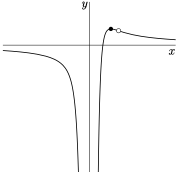
\includegraphics{graphE10b}
\begin{tikzpicture}
\YEaaxis{5}{5}{4}{1}
\draw[thick, red] plot[domain=-5:-1.15](\x,{2*(\x*\x*\x-2)/(\x*\x*\x*\x)});
\draw[thick, red] plot[domain=.9:5](\x,{2*(\x*\x*\x-2)/(\x*\x*\x*\x)});
\draw (2.7,0.65) node[opendot]{};
\draw (2,.75) node[vertex, label=above:{$\left(2,\frac{3}{8}\right)$}]{};
\YExcoord{2}{2}
\YExcoord{2.7}{\sqrt[3]{20}}
\YExcoord{1.3}{\sqrt[3]{2}}
\end{tikzpicture}
\end{center}
\end{answer}
\begin{hint}
The local maximum is also a global maximum.
\end{hint}
\begin{solution}
\begin{itemize}
\item Asymptotes:
\[\ds\lim_{x \to \pm \infty}f(x) = \ds\lim_{x \to \pm \infty}\dfrac{1}{x}-\dfrac{2}{x^4}=0\]
So $y=0$ is a horizontal asymptote both at $x=\infty$ and
$x=-\infty$.

\[\ds\lim_{x \to0}f(x) = \ds\lim_{x \to 0}\dfrac{x^3-2}{x^4}=-\infty\]
So there is a vertical asymptote at  $x=0$, where the function plunges downwards from both the right and the left.

\item Intervals of increase and decrease:

\[f'(x)=-\frac{1}{x^2}+\frac{8}{x^5}=\frac{8-x^3}{x^5}\]
The only place where $f'(x)$ is zero only at $x=2$. So $f(x)$ has a horizontal tangent at $x=2$,
$y=\frac{3}{8}$. This is a critical point.

The derivative is undefined at $x=0$, as is the function.

\begin{center}
 \begin{tabular}{|c||c|c|c|c|c|}
\hline
$x$  & $(-\infty,0)$ &$0$ & $(0,2)$ & $2$&$(2,\infty)$ \\
\hline
$f'(x)$  & negative  & DNE & positive & 0&  negative\\
\hline
$f(x)$ & decreasing & vertical asymptote & increasing &local max & decreasing\\
\hline
 \end{tabular}
\end{center}

Since the function changes from increasing to decreasing at $x=2$, the only local maximum is at $x=2$.

At this point, we get a rough sketch of $f(x)$.
\begin{center}
\begin{tikzpicture}
\YEaaxis{5}{5}{4}{1}
\draw[thick] (-4.5,-.25)--(-1,-.5)--(-.5,-4);
\draw[thick] (.5,-4)--(2,1)--(4.5,.25);
\YExcoord{2}{2}
\draw[thick, <-, orange] (-4,1)--(-2,2.5) ;
\draw[orange] (0,3)node{horizontal asymptotes $y=0$};
\draw[thick, <-, orange] (4,1)--(2,2.5);
\draw[blue, decorate, decoration={brace, amplitude=10pt, mirror}] (-5,-4.25)--(0,-4.25);
\draw[blue] (-2.5,-5)node{decreasing};
\draw[blue, decorate, decoration={brace, amplitude=10pt, mirror}] (2,-4.25)--(5,-4.25);
\draw[blue] (3.5,-5)node{decreasing};
\draw[red, decorate, decoration={brace, amplitude=10pt, mirror}] (0,-4.25)--(2,-4.25);
\draw[red] (1,-5)node{increasing};
\draw (2,1) node[vertex, label=above:{$\left(2,\frac{3}{8}\right)$}]{};
\end{tikzpicture}
\end{center}
%\item Global extrema:
%
%Since $\ds\lim_{x \to -\infty}f(x)=0$ and $f(x)$ is deceasing on $(-\infty, 0)$, we conclude $f(x)\le0$ for all $-\infty<x<0$.

\item Concavity:
\[f''(x)=\frac{2}{x^3}-\frac{40}{x^6}=\frac{2x^3-40}{x^6}\]
The second derivative of $f(x)$ is positive for $x>\root 3\of 20$ and negative for $x<\root 3\of 20$.
So the curve is concave up for $x>\root 3\of 20$ and concave down for
$x<\root 3\of 20$. There is an inflection point at $x=\root 3\of 20\approx 2.7$,
$y=\frac{18}{20^{4/3}}\approx 0.3$.

\item Intercepts:

Since $f(x)$ is not defined at $x=0$, there is no $y$-intercept. The only $x$-intercept is $x=\sqrt[3]{2}\approx 1.3$.

\item Sketch:


We can add concavity to our skeleton sketched above, and label our intercept and inflection point (the open dot).
\begin{center}
\begin{tikzpicture}
\YEaaxis{5}{5}{4}{1}
\draw[thick, red] plot[domain=-5:-1.15](\x,{2*(\x*\x*\x-2)/(\x*\x*\x*\x)});
\draw[thick, red] plot[domain=.9:5](\x,{2*(\x*\x*\x-2)/(\x*\x*\x*\x)});
\draw (2.7,0.65) node[opendot]{};
\draw (2,.75) node[vertex, label=above:{$\left(2,\frac{3}{8}\right)$}]{};
\YExcoord{2}{2}
\YExcoord{2.7}{\sqrt[3]{20}}
\YExcoord{1.3}{\sqrt[3]{2}}
\draw[blue, decorate, decoration={brace, amplitude=10pt, mirror}] (-5,-4.25)--(0,-4.25);
\draw[blue] (-2.5,-5)node{decreasing};
\draw[blue, decorate, decoration={brace, amplitude=10pt, mirror}] (2,-4.25)--(5,-4.25);
\draw[blue] (3.5,-5)node{decreasing};
\draw[red, decorate, decoration={brace, amplitude=10pt, mirror}] (0,-4.25)--(2,-4.25);
\draw[red] (1,-5)node{increasing};
\draw[blue, decorate, decoration={brace, amplitude=10pt, mirror}] (-5,-5.5)--(2.7,-5.5);
\draw[blue] (-1,-6.25)node{concave down};
\draw[red, decorate, decoration={brace, amplitude=10pt, mirror}] (2.7,-5.5)--(5,-5.5);
\draw[red] (4,-6.25)node{concave up};
\end{tikzpicture}
\end{center}
\end{itemize}
%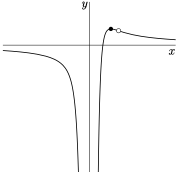
\includegraphics{graphE10b}
\end{solution}


\begin{question}[1997A]
The first and second derivatives of the function $f(x)=\dfrac{x^4}{1+x^3}$ are:
$$
f'(x)=\frac{4x^3+x^6}{(1+x^3)^2}\qquad\hbox{and}\qquad f''(x)=\frac{12x^2-6x^5}{(1+x^3)^3}
$$
Graph $f(x)$. Include local
and absolute maxima and minima, regions where $f(x)$ is increasing or
decreasing, regions where the curve is concave upward
or downward, and any asymptotes.
\end{question}
\begin{hint}
The sign of the first derivative is determined entirely by the numerator, but the sign of the second derivative depends on both the numerator and the denominator.
\end{hint}
\begin{answer}
The open dot marks the inflection point.
\begin{center}\begin{tikzpicture}
\YEaxis{6}{4}
\draw plot[domain=-3:-1.1, samples=50](2*\x,{\x*\x*\x*\x/(1+\x*\x*\x)});
\draw plot[domain=-0.93:3, samples=100](2*\x,{\x*\x*\x*\x/(1+\x*\x*\x)});
\draw[dashed](-2,-4)--(-2,-.75) (-2,.5)--(-2,4);
\YExcoord{-2}{-1}
\YExcoord{-3.2}{-\sqrt[3]{4}}
\YExcoord{2.52}{\sqrt[3]{2}}
\draw (2.53,0.84) node[opendot]{};
\draw (0,0) node[vertex]{};
\draw (-3.2,-2.12) node[vertex]{};
\end{tikzpicture}\end{center}
\end{answer}
\begin{solution}
\begin{itemize}
\item  Asymptotes:

When $x=-1$, the denominator $1+x^3$ of $f(x)$ is zero while the numerator is 1,  so $x=-1$ is a vertical asymptote. More precisely,
\[\lim_{x \to -1^-}f(x)=-\infty
\qquad
\lim_{x \to -1^+}f(x)=\infty\]

There are no horizontal asymptotes, because
\[\lim_{x \to \infty} \frac{x^4}{1+x^3}=\infty \qquad \lim_{x \to- \infty} \frac{x^4}{1+x^3}=-\infty\]

\item  Intervals of increase and decrease:

We note that $f'(x)$ is defined for all $x \neq -1$, so $f'(x)$ is defined for all $x$ in the domain of $f(x)$. Therefore, $f(x)$ has no singular points.

To find critical points, we set
\begin{align*}
f'(x)&=0\\
4x^3+x^6 &=0\\
x^3(4+x^3)&=0\\
x^3=0 \qquad &\mbox{or} \qquad 4+x^3=0\\
x=0 \qquad &\mbox{or} \qquad x=-\sqrt[3]{4}\approx-1.6
\end{align*}

At these critical points, $f(0)=0$ and
$f(-\root 3 \of 4)=\frac{4\root 3 \of 4}{-3}<0$.
The denominator of $f'(x)$ is never negative, so the sign of $f'(x)$ is the same as the sign of its numerator, $x^3(4+x^3)$.

\begin{center}
 \begin{tabular}{|c||c|c|c|c|c|c|c|}
\hline
$x$  & $(-\infty,-\sqrt[3]{4})$ &$-\sqrt[3]{4}$ & $(-\sqrt[3]{4},-1)$ & $-1$ &$(-1,0)$
&$0$&$(0,\infty)$\\
\hline
$f'(x)$  &  positive &0  &negative  &DNE &negative &0&positive \\
\hline
$f(x)$ & increasing & l. max&decreasing&VA &decreasing&l. min&increasing\\
\hline
 \end{tabular}
\end{center}

Now, we have enough information to make a skeleton of our graph.
\begin{center}\begin{tikzpicture}
\YEaxis{6}{4}
\YExcoord{-2}{-1}
\draw[dashed](-2,-4)--(-2,-.75) (-2,.5)--(-2,4);
\YExcoord{-3.2}{-\sqrt[3]{4}}
\draw[thick] (-6,-4)--(-3.2,-1)--(-2.3,-2)--(-2.1,-4);
\draw[thick] (-1.9,4)--(-1.7,2)--(0,0)--(6,4);
\draw[red, decorate, decoration={brace, amplitude=10pt, mirror}] (-6,-4.25)--(-3.2,-4.25);
\draw[red] (-4.8,-5)node{increasing};
\draw[blue, decorate, decoration={brace, amplitude=8pt, mirror}] (-3.2,-4.25)--(-2,-4.25);
\draw[blue] (-2.6,-5)node{decr};
\draw[blue, decorate, decoration={brace, amplitude=10pt, mirror}] (-2,-4.25)--(0,-4.25);
\draw[blue] (-1,-5)node{decr};
\draw[red, decorate, decoration={brace, amplitude=10pt, mirror}] (0,-4.25)--(6,-4.25);
\draw[red] (3,-5)node{increasing};
\end{tikzpicture}\end{center}

\item Concavity:

The second derivative is undefined when $x=-1$. It is zero when $12x^2-6x^5=6x^2(2-x^3)=0$.
That is, at $x=\root 3\of 2\approx 1.3$ and $x=0$.  Notice that the sign of $f''(x)$ does not change at $x=0$, so $x=0$ is not an inflection point.


\begin{center}
 \begin{tabular}{|c||c|c|c|c|c|c|c|}
\hline
$x$  & $(-\infty,-1)$ &$-1$ & $(-1,0)$ & $0$ &$(0,\sqrt[3]{2})$
&$\sqrt[3]{2}$&$(\sqrt[3]{2},\infty)$\\
\hline
$f''(x)$  &  negative &DNE  &positive  &0 &positive &0&negative \\
\hline
$f(x)$ & concave down & VA&concave up&&concave up&IP&concave down\\
\hline
 \end{tabular}
\end{center}

Now we can refine our skeleton by adding concavity.
\begin{center}\begin{tikzpicture}
\YEaxis{6}{4}
\draw plot[domain=-3:-1.1, samples=50](2*\x,{\x*\x*\x*\x/(1+\x*\x*\x)});
\draw plot[domain=-0.93:3, samples=100](2*\x,{\x*\x*\x*\x/(1+\x*\x*\x)});
\draw[dashed](-2,-4)--(-2,-.75) (-2,.5)--(-2,4);
\YExcoord{-2}{-1}
\YExcoord{-3.2}{-\sqrt[3]{4}}
\YExcoord{2.52}{\sqrt[3]{2}}
\draw[red, decorate, decoration={brace, amplitude=10pt, mirror}] (-6,-4.25)--(-3.2,-4.25);
\draw[red] (-4.8,-5)node{increasing};
\draw[blue, decorate, decoration={brace, amplitude=8pt, mirror}] (-3.2,-4.25)--(-2,-4.25);
\draw[blue] (-2.8,-5)node{decr};
\draw[blue, decorate, decoration={brace, amplitude=10pt, mirror}] (-2,-4.25)--(0,-4.25);
\draw[blue] (-1,-5)node{decr};
\draw[red, decorate, decoration={brace, amplitude=10pt, mirror}] (0,-4.25)--(6,-4.25);
\draw[red] (3,-5)node{increasing};
\draw[blue, decorate, decoration={brace, amplitude=10pt, mirror}] (-6,-5.5)--(-2,-5.5);
\draw[blue] (-4,-6.25)node{concave down};
\draw[red, decorate, decoration={brace, amplitude=10pt, mirror}] (-2,-5.5)--(2.5,-5.5);
\draw[red] (0.25,-6.25)node{concave up};
\draw[blue, decorate, decoration={brace, amplitude=10pt, mirror}] (2.5,-5.5)--(6,-5.5);
\draw[blue] (4.25,-6.25)node{concave down};

\draw (2.53,0.84) node[opendot]{};
\draw (0,0) node[vertex]{};
\draw (-3.2,-2.12) node[vertex]{};
\end{tikzpicture}\end{center}
\end{itemize}
%\begin{center}
%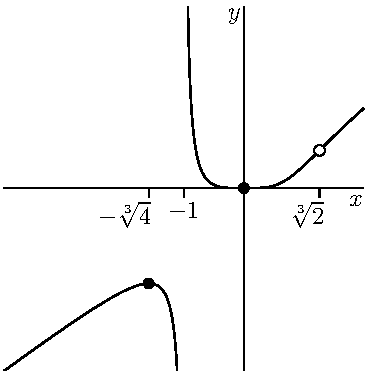
\includegraphics{graphW58}\end{center}
\end{solution}


\begin{Mquestion}[1996D]\label{s3.6.6rationallast}
 The first and second derivatives of the function $f(x)=\dfrac{x^3}{1-x^2}$ are:
$$
f'(x)=\frac{3x^2-x^4}{(1-x^2)^2}\qquad\hbox{and}\qquad f''(x)=\frac{6x+2x^3}{(1-x^2)^3}
$$
Graph $f(x)$. Include local
and absolute maxima and minima, regions where the curve is concave upward
or downward, and any asymptotes.
\end{Mquestion}
\begin{hint}
The function is odd.
\end{hint}
\begin{answer}
\begin{center}
%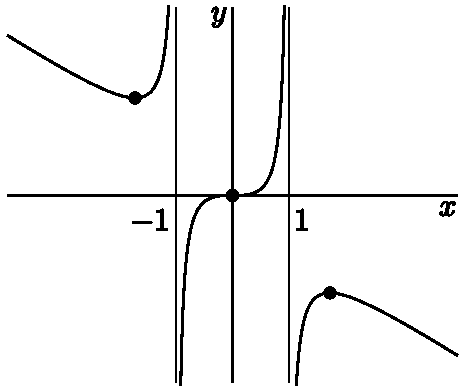
\includegraphics{graphE5}
\begin{tikzpicture}
\YEaxis{6}{4}
\draw plot[domain=-3:-1.08, samples=50](2*\x,{\x*\x*\x/(1-\x*\x)/2});
\draw plot[domain=-.945:.945, samples=50](2*\x,{\x*\x*\x/(1-\x*\x)/2});
\draw plot[domain=1.08:3, samples=50](2*\x,{\x*\x*\x/(1-\x*\x)/2});
\YExcoord{-2}{-1}
\YExcoord{2}{1}
\YExcoord{-3.46}{-\sqrt{3}}
\YExcoord{3.46}{\sqrt{3}}
\YEycoord{1.3}{\frac{3\sqrt{3}}{2}}
\YEycoord{-1.3}{-\frac{3\sqrt{3}}{2}}
\draw[dashed] (-2,-4)--(-2,-1) (-2,.5)--(-2,4);
\draw[dashed] (2,-4)--(2,-1) (2,.5)--(2,4);
\draw(-3.46,1.3) node[vertex]{};
\draw(3.46,-1.3) node[vertex]{};
\draw(0,0) node[opendot]{};
\end{tikzpicture}
\end{center}
\end{answer}
\begin{solution}
\begin{itemize}
\item Asymptotes:
\[\lim_{x \to -\infty}\frac{x^3}{1-x^2}=\infty \qquad
\lim_{x \to \infty}\frac{x^3}{1-x^2}=-\infty \]
So, $f(x)$ has no horizontal asymptotes.

 On the other hand $f(x)$ blows up at both $x=1$
and $x=-1$, so there are vertical asymptotes at $x=1$ and $x=-1$.
More precisely,
\begin{align*}
\lim_{x \to -1^-}\frac{x^3}{1-x^2}&=\infty
&
\lim_{x \to -1^+}\frac{x^3}{1-x^2}&=-\infty\\
\lim_{x \to 1^-}\frac{x^3}{1-x^2}&=\infty
&
\lim_{x \to 1^+}\frac{x^3}{1-x^2}&=-\infty
\end{align*}

\item Symmetry:

$f(x)$ is an odd function, because
\[f(-x)=\frac{(-x)^3}{1-(-x)^2}=\frac{-x^3}{1-x^2}=-f(x)\]

\item Intercepts:

The only intercept of $f(x)$ is the origin. In particular, that means that out of the three intervals where it is continuous,
                  namely $(-\infty,-1)$, $(-1,1)$ and $(1,\infty)$, in two of them $f(x)$ is always positive or always negative.
\begin{itemize}
\item When $x<-1$:\quad $1-x^2<0$ and $x^3<0$, so $f(x)>0$.
\item When $x>1$:\qquad $1-x^2<0$ and $x^3>0$, so $f(x)<0$.
\item When $-1<x<0$, $1-x^2>0$ and $x^3<0$ so $f(x)<0$.
\item When $0<x<1$, $1-x^2>0$ and $x^3>0$ so $f(x)>0$.
\end{itemize}

\item Intervals of increase and decrease:

\[f'(x)=\dfrac{3x^2-x^4}{(1-x^2)^2}=\frac{x^2(3-x^2)}{(1-x^2)^2}\]
There are no singular points (but remember the domain of $f(x)$ does not include $x=\pm 1$ ). The critical points are:
\begin{align*}
f'(x)&=0\\
x^2=0\qquad&\mbox{or}\qquad 3-x^2=0\\
x=0\qquad&\mbox{or}\qquad x=\pm\sqrt{3}\approx\pm 1.7
\end{align*}

The values of $f$ at its critical points are
$f(0)=0$, $f(\sqrt{3})=-\dfrac{3\sqrt{3}}{2}\approx -2.6$ and $f(-\sqrt{3})=\dfrac{3\sqrt{3}}{2}\approx2.6$.

Notice the sign of $f'(x)$ is the same as the sign of $3-x^2$.

\begin{center}
 \begin{tabular}{|c||c|c|c|c|c|c|c|}
\hline
$x$  & $(-\infty,-\sqrt{3})$ &$-\sqrt{3}$&$(-\sqrt 3,-1)$&$-1$\\
\hline
$f'(x)$  &negative&0&positive&DNE\\
\hline
$f(x)$ & decreasing&local min&increasing&VA\\
\hline
 \end{tabular}

 \begin{tabular}{|c||c|c|c|c|c|c|c|}
\hline
$x$  & $(-1,0)$ &$0$&$(0,\sqrt 3)$&$\sqrt{3}$&$(\sqrt{3},\infty)$\\
\hline
$f'(x)$  &positive&0&positive&0&negative\\
\hline
$f(x)$ &increasing & & increasing & local max & decreasing \\
\hline
 \end{tabular}
\end{center}

Now we have enough information to sketch a skeleton of $f(x)$.

\begin{center}
\begin{tikzpicture}
\YEaxis{6}{4}
\YExcoord{-2}{-1}
\YExcoord{2}{1}
\YExcoord{-3.46}{-\sqrt{3}}
\YExcoord{3.46}{\sqrt{3}}
\YEycoord{1.3}{\frac{3\sqrt{3}}{2}}
\YEycoord{-1.3}{-\frac{3\sqrt{3}}{2}}
\draw[dashed] (-2,-4)--(-2,-1) (-2,.5)--(-2,4);
\draw[dashed] (2,-4)--(2,-1) (2,.5)--(2,4);
\draw[blue, decorate, decoration={brace, amplitude=10pt, mirror}] (-6,-4.25)--(-3.46,-4.25);
\draw[blue] (-4.75,-5) node{decreasing};
\draw[red, decorate, decoration={brace, amplitude=10pt, mirror}] (-3.46,-4.25)--(-2,-4.25);
\draw[red] (-2.75,-5) node{incr};
\draw[red, decorate, decoration={brace, amplitude=10pt, mirror}] (-2,-4.25)--(2,-4.25);
\draw[red] (0,-5) node{increasing};
\draw[red, decorate, decoration={brace, amplitude=10pt, mirror}] (2,-4.25)--(3.46,-4.25);
\draw[red] (2.75,-5) node{incr};
\draw[blue, decorate, decoration={brace, amplitude=10pt, mirror}] (3.46,-4.25)--(6,-4.25);
\draw[blue] (4.75,-5) node{decreasing};
\draw(-3.46,1.3) node[vertex]{};
\draw(3.46,-1.3) node[vertex]{};
\draw(0,0) node[vertex]{};
\draw[thick] (-6,4)--(-3.46,1.3)--(-2.2,2)--(-2.1,4);
\draw[thick] (6,-4)--(3.46,-1.3)--(2.2,-2)--(2.1,-4);
\draw[thick] (-1.9,-4)--(-1.8,-1)--(-.5,0)--(.5,0)--(1.8,2)--(1.9,4);
\end{tikzpicture}
\end{center}

\item Concavity:
\[f''(x)=\frac{2x(3+x^2)}{(1-x^2)^3}\]

The second derivative is zero when $x=0$, and is undefined when $x=\pm 1$.

\begin{center}
 \begin{tabular}{|c||c|c|c|c|c|c|c|}
\hline
$x$  & $(-\infty,-1)$ &$(-1,0)$&0&$(0,1)$&$(1,\infty)$\\
\hline
$f''(x)$  &positive&negative&0&positive&negative\\
\hline
$f(x)$ & concave up&concave down&inflection point&concave up&concave down\\
\hline
 \end{tabular}
\end{center}
Now, we can refine our skeleton.

\begin{center}
\begin{tikzpicture}
\YEaxis{6}{4}
\draw plot[domain=-3:-1.08, samples=50](2*\x,{\x*\x*\x/(1-\x*\x)/2});
\draw plot[domain=-.945:.945, samples=50](2*\x,{\x*\x*\x/(1-\x*\x)/2});
\draw plot[domain=1.08:3, samples=50](2*\x,{\x*\x*\x/(1-\x*\x)/2});
\YExcoord{-2}{-1}
\YExcoord{2}{1}
\YExcoord{-3.46}{-\sqrt{3}}
\YExcoord{3.46}{\sqrt{3}}
\YEycoord{1.3}{\frac{3\sqrt{3}}{2}}
\YEycoord{-1.3}{-\frac{3\sqrt{3}}{2}}
\draw[dashed] (-2,-4)--(-2,-1) (-2,.5)--(-2,4);
\draw[dashed] (2,-4)--(2,-1) (2,.5)--(2,4);
\draw(-3.46,1.3) node[vertex]{};
\draw(3.46,-1.3) node[vertex]{};
\draw(0,0) node[opendot]{};

\draw[blue, decorate, decoration={brace, amplitude=10pt, mirror}] (-6,-4.25)--(-3.46,-4.25);
\draw[blue] (-4.75,-5) node{decreasing};
\draw[red, decorate, decoration={brace, amplitude=10pt, mirror}] (-3.46,-4.25)--(-2,-4.25);
\draw[red] (-2.75,-5) node{incr};
\draw[red, decorate, decoration={brace, amplitude=10pt, mirror}] (-2,-4.25)--(2,-4.25);
\draw[red] (0,-5) node{increasing};
\draw[red, decorate, decoration={brace, amplitude=10pt, mirror}] (2,-4.25)--(3.46,-4.25);
\draw[red] (2.75,-5) node{incr};
\draw[blue, decorate, decoration={brace, amplitude=10pt, mirror}] (3.46,-4.25)--(6,-4.25);
\draw[blue] (4.75,-5) node{decreasing};
\draw[red, decorate, decoration={brace, amplitude=10pt, mirror}] (-6,-5.5)--(-2,-5.5);
\draw[red] (-4,-6.25) node{concave up};
\draw[blue, decorate, decoration={brace, amplitude=10pt, mirror}] (-2,-5.5)--(0,-5.5);
\draw[blue] (-1,-6.25) node{cc down};
\draw[red, decorate, decoration={brace, amplitude=10pt, mirror}] (0,-5.5)--(2,-5.5);
\draw[red] (1,-6.25) node{concave up};
\draw[blue, decorate, decoration={brace, amplitude=10pt, mirror}] (2,-5.5)--(6,-5.5);
\draw[blue] (4,-6.25) node{concave down};
\end{tikzpicture}
\end{center}
%\begin{center}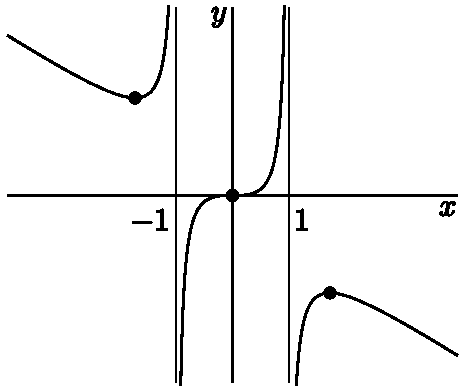
\includegraphics{graphE5}\end{center}
\end{itemize}
\end{solution}






\begin{Mquestion}[2006H]
The function $f(x)$ is defined by
\[
f(x) =
\left\{\begin{array}{lc}
e^x &x<0\\
 \frac{x^2+3}{3(x+1)} & x \ge 0
 \end{array}\right.
\]
\begin{enumerate}[(a)]
\item\label{s3.6_2006_a} Explain why $f(x)$ is continuous everywhere.
\item\label{s3.6_2006_b} Determine all of the following if they are present:

\begin{enumerate}[i.]
\item\label{s3.6_2006_i} $x$--coordinates of local maxima and minima, intervals
          where $f(x)$ is increasing or decreasing;
\item\label{s3.6_2006_ii} intervals where $f(x)$ is concave upwards or downwards;
\item\label{s3.6_2006_iii} equations of any horizontal or vertical asymptotes.
\end{enumerate}

\item\label{s3.6_2006_c} Sketch the graph of $y = f(x)$, giving the $(x, y)$
coordinates for all points of interest above.
\end{enumerate}
\end{Mquestion}
\begin{hint}
The function is continuous at $x=0$, but its derivative is not.
\end{hint}
\begin{answer}
\eqref{s3.6_2006_a}
One branch of the function,
the exponential function $e^x$, is continuous everywhere. So $f(x)$ is continuous for $x<0$. When $x \geq 0$, $f(x)=\dfrac{x^2+3}{3(x+1)}$, which is continuous whenever $x \neq -1$ (so it's continuous for all $x >0$). So, $f(x)$ is continuous for $x>0$. To see that $f(x)$ is continuous at $x=0$, we see:
\begin{align*}
\lim_{x\rightarrow0-}f(x)=\lim_{x\rightarrow0-}e^x&=1\\
\lim_{x\rightarrow0+}f(x)=\lim_{x\rightarrow0+}\frac{x^2+3}{3(x+1)}&=1\\
\mbox{So, }~\lim_{x \rightarrow 0}f(x)&=1=f(0)
\end{align*}
Hence $f(x)$ is continuous at $x=0$, so $f(x)$ is continuous everywhere.\\
\eqref{s3.6_2006_b}
i.\\  $f(x)$ is increasing for $x<0$ and $x>1$, decreasing for $0<x<1$,
            has a local max at $(0,1)$, and has a local min at $\left(1,\frac{2}{3}\right)$.\\
ii.\\ $f(x)$ is concave upwards for all $x\ne 0$.\\
iii.\\ The $x$--axis is a horizontal asymptote as $x\rightarrow-\infty$.

\eqref{s3.6_2006_c}
%\centerline{\figput{OE06D_3}}
\begin{center}\begin{tikzpicture}
\YEaaxis{3}{3}{.5}{2}
\draw[thick] plot[domain=-3:0](\x,{exp(\x)});
\draw (0,1) node[vertex, label=above left:{$(0,1)$}]{};
\draw[thick] plot[domain=0:3](\x,{(\x*\x+3)/(3*\x+3)});
\draw (1,2/3) node[vertex, label=above:{$(1,\frac{2}{3})$}]{};
\end{tikzpicture}\end{center}
\end{answer}
\begin{solution}
\eqref{s3.6_2006_a}
One branch of the function,
the exponential function $e^x$, is continuous everywhere. So $f(x)$ is continuous for $x<0$. When $x \geq 0$, $f(x)=\dfrac{x^2+3}{3(x+1)}$, which is continuous whenever $x \neq -1$ (so it's continuous for all $x >0$). So, $f(x)$ is continuous for $x>0$. To see that $f(x)$ is continuous at $x=0$, we see:
\begin{align*}
\lim_{x\rightarrow0-}f(x)=\lim_{x\rightarrow0-}e^x&=1\\
\lim_{x\rightarrow0+}f(x)=\lim_{x\rightarrow0+}\frac{x^2+3}{3(x+1)}&=1\\
\mbox{So, }~\lim_{x \rightarrow 0}f(x)&=1=f(0)
\end{align*}
Hence $f(x)$ is continuous at $x=0$, so $f(x)$ is continuous everywhere.\\
\eqref{s3.6_2006_b}
We differentiate the function twice.
 Notice
 \begin{align*}
 \diff{}{x}\left\{\dfrac{x^2+3}{3(x+1)}\right\}&=\frac{3(x+1)(2x)-(x^2+3)(3)}{9(x+1)^2}\\
&=\frac{x^2+2x-3}{3(x+1)^2}\\
 &=\frac{(x-1)(x+3)}{3(x+1)^2}\qquad\mbox{where $x \neq -1$}\\
 \mbox{Then}\qquad
  \lim_{x \to 0^+}f'(x)&=\frac{(0-1)(0+3)}{3(0+1)^2}=-1 \neq 1 =e^0= \lim_{x \to 0^-}f'(x)\\
 \mbox{so}\qquad
f'(x)&=\left\{\begin{array}{ll}
e^x&x<0\\
DNE&x=0\\
\frac{(x-1)(x+3)}{3(x+1)^2}&x > 0
\end{array}\right.\\
 \intertext{Differentiating again,}
 \diff{^2}{x^2}\left\{\dfrac{x^2+3}{3(x+1)}\right\}&=
 \diff{}{x}\left\{\frac{x^2+2x-3}{3(x+1)^2}
 \right\}\\
 &=\frac{3(x+1)^2(2x+2)-(x^2+2x-3)(6)(x+1)}{9(x+1)^4}\left(\frac{\div3(x+1)}{\div3(x+1)}\right)\\
 &=\frac{(x+1)(2x+2)-2(x^2+2x-3)}{3(x+1)^3}\\
 &=\frac{8}{3(x+1)^3}\qquad\mbox{where $x \neq -1$}\\
 \mbox{so}\qquad
f''(x)&=\left\{\begin{array}{ll}
e^x&x<0\\
DNE&x=0\\
\frac{8}{3(x+1)^3}&x > 0
\end{array}\right.
 \end{align*}

i.
The only singular point is $x=0$, and the only critical point is $x=1$. (When you're reading off the expression for $f'(x)$, remember that the bottom line only applies when $x>0$.)
\begin{center}
\begin{tabular}{|c||c|c|c|c|c|}
\hline
$x$&$(-\infty,0)$&$0$&$(0,1)$&1&$(1,\infty)$\\
\hline
$f'(x)$&positive&DNE&negative&0&positive\\
\hline
$f(x)$&increasing&local max&decreasing&local min&increasing\\
\hline
\end{tabular}
\end{center}
The coordinates of the local maximum are $(0,1)$
and the coordinates of the local minimum are $\left(1,\frac{2}{3}\right)$.

ii.\\  When $x \neq 0$, $f''(x)$ is always positive, so $f(x)$ is concave up.\\
iii.\\
\begin{align*}
\lim_{x \to \infty} f(x)&=\lim_{x \to \infty} \frac{x^2+3}{3x+3}\\
&=\lim_{x \to \infty}\frac{x+\frac{3}{x}}{1+\frac{3}{x}}=\infty
\intertext{So, there is no horizontal asymptote to the right.}
\lim_{x \to -\infty} f(x)&=\lim_{x \to -\infty}e^x=0
\intertext{So, $y=0$ is a horizontal asymptote to the left.}
\end{align*}
Since $f(x)$ is continuous everywhere, there are no vertical asymptotes.

\eqref{s3.6_2006_c}
%\centerline{\figput{OE06D_3}}
\begin{center}\begin{tikzpicture}
\YEaaxis{3}{3}{.5}{2}
\draw[thick] plot[domain=-3:0](\x,{exp(\x)});
\draw (0,1) node[vertex, label=above left:{$(0,1)$}]{};
\draw[thick] plot[domain=0:3](\x,{(\x*\x+3)/(3*\x+3)});
\draw (1,2/3) node[vertex, label=above:{$(1,\frac{2}{3})$}]{};
\draw[red, decorate, decoration={brace, amplitude=10pt, mirror}](-3,-.75)--(0,-.75);
\draw[red] (-1.5,-1.5) node{increasing};
\draw[blue, decorate, decoration={brace, amplitude=6pt, mirror}](0,-.75)--(1,-.75);
\draw[blue] (.5,-1.5) node{decr};
\draw[red, decorate, decoration={brace, amplitude=10pt, mirror}](1,-.75)--(3,-.75);
\draw[red] (2,-1.5) node{increasing};
\draw[red, decorate, decoration={brace, amplitude=10pt, mirror}](-3,-2)--(0,-2);
\draw[red] (-1.5,-2.75) node{concave up};
\draw[red, decorate, decoration={brace, amplitude=10pt, mirror}](0,-2)--(3,-2);
\draw[red] (1.5,-2.75) node{concave up};
\end{tikzpicture}\end{center}
\end{solution}


\Instructions{In Questions~\ref{s3.6.6expfirst} and \ref{s3.6.6explast}, you will sketch the graphs of functions with an exponential component. In the next section, you will learn how to find their horizontal asymptotes, but for now these are given to you.}

\begin{question}[1997D]\label{s3.6.6expfirst}
The function $f(x)$ and its derivative are given below:
\[
f(x)=(1+2x)e^{-x^2}\qquad\hbox{and}\qquad f'(x)=2(1-x-2x^2)e^{-x^2}
\]
Sketch the graph of $f(x)$. Indicate the critical points, local
and/or absolute maxima and minima, and asymptotes. Without actually calculating
the inflection points, indicate on the graph their approximate location.

Note: $\ds\lim_{x \to \pm\infty}f(x)=0$.
\end{question}
\begin{hint}
Since you aren't asked to find the intervals of concavity exactly, sketch the intervals of increase and decrease, and turn them into a smooth curve. You might not get exactly the intervals of concavity that are given in the solution, but there should be the same number of intervals as the solution, and they should have the same positions relative to the local extrema.
\end{hint}
\begin{answer}\begin{center}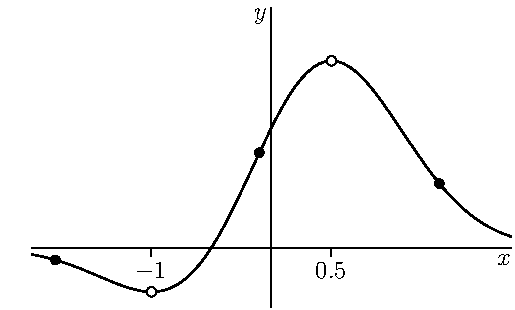
\includegraphics{graphE12}\end{center}
\end{answer}
\begin{solution}
\begin{itemize}
\item Asymptotes:
In the problem statement, we are told:
\[\lim_{x \to \pm \infty}\frac{1+2x}{e^{x^2}}=0\]
So, $y=0$ is a horizontal asymptote both at $x=\infty$ and at $x=-\infty$.

Since $f(x)$ is continuous, it has no vertical asymptotes.

\item Intervals of increase and decrease:

The critical points are the zeroes of $1-x-2x^2=(1-2x)(1+x)$. That is,
 $x=\frac{1}{2},\ -1$.

\begin{center}
\begin{tabular}{|c||c|c|c|c|c|}
\hline
$x$&$(-\infty,-1)$&$-1$&$(-1,\frac{1}{2})$&$\frac{1}{2}$&$(\frac{1}{2},\infty)$\\
\hline
$f'(x)$&negative&0&positive&0&negative\\
\hline
$f(x)$&decreasing&local min&increasing&local max&decreasing\\
\hline
\end{tabular}
\end{center}
At these critical points, $f\big(\frac{1}{2}\big)=2e^{-1/4}>0$ and $f(-1)=-e^{-1}<0$.

From here, we can sketch a skeleton of the graph.
\begin{center}
\begin{tikzpicture}
\YEaaxis{4.25}{4.25}{1}{3}
\YExcoord{-2}{-1}
\YExcoord{1}{\frac{1}{2}}
\draw[thick] (-4,-.1)--(-2,-.3)--(1,2)--(2,.5)--(4,.25);
\draw[blue, decorate, decoration={brace, amplitude=10pt, mirror}] (-4,-1)--(-2,-1);
\draw[blue] (-3,-1.75) node{decreasing};
\draw[red, decorate, decoration={brace, amplitude=10pt, mirror}] (-2,-1)--(1,-1);
\draw[red] (-.5,-1.75) node{increasing};
\draw[blue, decorate, decoration={brace, amplitude=6pt, mirror}] (1,-1)--(2,-1);
\draw[blue] (1.5,-1.75) node{decr};
\draw[red, decorate, decoration={brace, amplitude=10pt, mirror}] (2,-1)--(4,-1);
\draw[red] (3,-1.75) node{increasing};
%\draw[thick] plot[domain=-2:2](2*\x,{(1+2*\x)/(exp(\x*\x))});
\end{tikzpicture}
\end{center}

\item Concavity:

We are told that we don't have to actually solve for the inflection points. We just need to know enough to get a basic idea. So, we'll turn the skeleton of the graph into smooth curve.

\begin{center}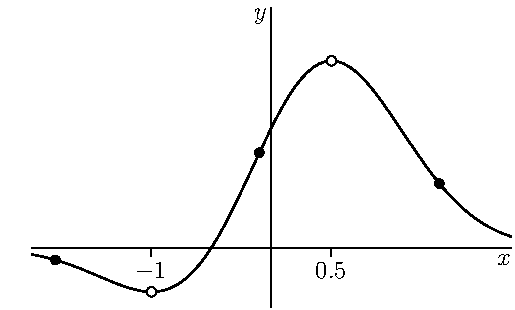
\includegraphics{graphE12}\end{center}

Inflection points are points where the convexity changes from up
to down or vice versa. It looks like our graph is convex down for $x$ from
$-\infty$ to about $-1.8$, convex up from about $x=-1.8$ to about $x=-0.1$,
convex down from about $x=-0.1$ to about $x=1.4$ and convex up from about
$x=1.4$ to infinity. So there are three inflection points at roughly
$x=-1.8,\ -0.1,\ 1.4$.
\end{itemize}
\end{solution}


\begin{Mquestion}[2009H]\label{s3.6.6explast}
Consider the function $f(x) = xe^{-x^2/2}$.

Note: $\ds\lim_{x \to \pm\infty}f(x)=0$.
\begin{enumerate}[(a)]
%\item\label{s3.62009_1} Find $\ds\lim_{x \to \infty}f(x)$ and $\ds\lim_{x \to -\infty}f(x)$.
\item\label{s3.62009_2} Find all inflection points and intervals of increase, decrease,
 convexity up, and convexity down. \\You may use without proof the formula
$f''(x) = (x^3-3x)e^{-x^2/2}$.
\item\label{s3.62009_3} Find local and global minima and maxima.
\item\label{s3.62009_4}  Use all the above to draw a graph for $f$. Indicate all
special points on the graph.
\end{enumerate}
\end{Mquestion}
\begin{hint}
Use intervals of increase and decrease, concavity, and asymptotes to sketch the curve.
\end{hint}
\begin{answer}
\eqref{s3.62009_2}
Increasing: $(-1,1)$\qquad decreasing: $(-\infty,-1)\cup (1,\infty)$\\
concave up: $(-\sqrt{3},0) \cup (\sqrt{3},\infty)$\qquad concave down: $(-\infty,-\sqrt{3}) \cup (0 ,\sqrt{3})$\\
inflection points: $x=\pm\sqrt{3}, 0$

\eqref{s3.62009_3}
The local and global minimum of $f(x)$ is at $(-1,\frac{-1}{\sqrt{e}})$, and the local and global maximum of $f(x)$ is at $(1,\frac{1}{\sqrt{e}})$.

\eqref{s3.62009_4}
In the graph below, open dots are inflection points, and
solid dots are extrema.
\begin{center}\begin{tikzpicture}
\YEaxis{6.5}{3};
\draw[thick] plot[domain=-3:3, scale=2, samples=100](\x,{2*\x*exp(-\x*\x/2)});
\draw (3.5,1.54) node[opendot]{};
\draw (-3.5,-1.53) node[opendot]{};
\YExcoord{-2}{-1}
\YExcoord{2}{1}
\draw (-3.5,.2) -- (-3.5,-.05) node[below]{$-\sqrt{3}$};
\YExcoord{3.5}{\sqrt{3}}
\YEycoord{-2.4}{\dfrac{-1}{\sqrt e}}
\YEycoord{2.4}{\dfrac{1}{\sqrt e}}
\draw (2,2.4) node[vertex]{};
\draw (-2,-2.4) node[vertex]{};
\end{tikzpicture}\end{center}
\end{answer}
\begin{solution}

\eqref{s3.62009_2}  We need to know the first and second derivative of $f(x)$. Using the product and chain rules, $f'(x)=e^{-x^2/2}(1-x^2)$. Given to us is $f''(x) = (x^3-3x)e^{-x^2/2}$. (These derivatives are also easy to find using the formula developed in Question~\ref{s2.14expprod}, Section~\ref*{sec higher diff}.)%2.14, higher order derivatives

Since $e^{-x^2/2}$ is always positive, the sign of $f'(x)$ is the same as the sign of $1-x^2$. $f(x)$ has no singular points and its only critical points are $x=\pm 1$. At these critical points, $f(-1)=-\dfrac{1}{\sqrt{e}}$ and $f(1)=\dfrac{1}{\sqrt{e}}$.
\begin{center}
\begin{tabular}{|c||c|c|c|c|c|}
\hline
$x$&$(-\infty,-1)$&$-1$&$(-1,1)$&$1$&$(1,\infty)$\\
\hline
$f'(x)$&negative&0&positive&0&negative\\
\hline
$f(x)$&decreasing&local min&increasing&local max&decreasing\\
\hline
\end{tabular}
\end{center}

This, together with the observations that $f(x)<0$ for $x<0$,
          $f(0)=0$ and $f(x)>0$ for $x>0$ (in fact $f$ is an odd function),
          is enough to sketch a skeleton of our graph.

\begin{center}\begin{tikzpicture}
\YEaxis{5}{2};
\draw (-2,.2) -- (-2,-.2) node[below]{$-1$};
\draw (2,.2) -- (2,-.2) node[below]{$1$};
\draw (.2,-1)--(-.2,-1) node[left]{$-\frac{1}{\sqrt{e}}$};
\draw (.2,1)--(-.2,1) node[left]{$\frac{1}{\sqrt{e}}$};
\draw[ thick] (-5,-.1)-- (-4,-.2)--(-2,-1);
\draw[thick] (-2,-1)--(2,1);
\draw[thick] (2,1)--(4,.2)--(5,.1);
\end{tikzpicture}\end{center}


We can factor $f''(x) = (x^3-3x)e^{-x^2/2}=x(x+\sqrt{3})(x-\sqrt{3})e^{-x^2/2}$. Since $e^{-x^2/2}$ is always positive, the sign of $f''(x)$ is the same as the sign of $x(x+\sqrt{3})(x-\sqrt{3})$.

\begin{center}
\begin{tabular}{|c||c|c|c|c|c|c|c|}
\hline
$x$&$(-\infty,-\sqrt{3})$&$-\sqrt{3}$&$(-\sqrt{3},0)$
&0&$(0,\sqrt{3})$
&$\sqrt{3}$&$(\sqrt{3},\infty)$\\
\hline
$f''(x)$&negative&0&positive&0&negative&0&positive\\
\hline
$f(x)$&concave down&IP&concave up&IP&concave down&IP&concave up\\
\hline
\end{tabular}
\end{center}

\eqref{s3.62009_3} We've already seen that $f(x)$ has a local min at $x=-1$ and a local max at $x=1$.

As $x$ tends to negative infinity, $f(x)$ tends to 0, and $f(x)$ is decreasing on $(-\infty,-1)$. Then $f(x)$ is between $0$ and $f(-1)=\frac{-1}{\sqrt{e}}$ on $(-\infty,-1)$. Then $f(x)$ is increasing on $(-1,1)$ from $f(-1)=\frac{-1}{\sqrt{e}}$ to $f(1)=\frac{1}{\sqrt{e}}$. Finally, for $x>1$, $f(x)$ is decreasing from $f(1)=\frac{1}{\sqrt{e}}$ and tending to 0. So when $x>1$, $f(x)$ is between $\frac{1}{\sqrt{e}}$ and $0$.

So, over its entire domain, $f(x)$ is between $\frac{-1}{\sqrt{e}}$ and $\frac{1}{\sqrt{e}}$, and it only achieves those values at $x=-1$ and $x=1$, respectively. Therefore, the local and global min of $f(x)$ is at $(-1,\frac{-1}{\sqrt{e}})$, and the local and global max of $f(x)$ is at $(1,\frac{1}{\sqrt{e}})$.

\eqref{s3.62009_4}
In the graph below, open dots are inflection points, and
solid dots are extrema.
\begin{center}\begin{tikzpicture}
\YEaxis{6.5}{3};
\draw[thick] plot[domain=-3:3, scale=2, samples=100](\x,{2*\x*exp(-\x*\x/2)});
\draw (3.5,1.54) node[opendot]{};
\draw (-3.5,-1.53) node[opendot]{};
\YExcoord{-2}{-1}
\YExcoord{2}{1}
\draw (-3.5,.2) -- (-3.5,-.05) node[below]{$-\sqrt{3}$};
\YExcoord{3.5}{\sqrt{3}}
\YEycoord{-2.4}{\dfrac{-1}{\sqrt e}}
\YEycoord{2.4}{\dfrac{1}{\sqrt e}}
\draw (2,2.4) node[vertex]{};
\draw (-2,-2.4) node[vertex]{};
\end{tikzpicture}\end{center}
%\centerline{\figput{OE09D_4}}
\end{solution}

\Instructions{In Questions~\ref{s3.6.6trig1} and \ref{s3.6.6trig2}, you will sketch the graphs of functions that have a trigonometric component.}

\begin{question}\label{s3.6.6trig1}
Use the techniques from this section to sketch the graph of $f(x)=x+2\sin x$.
\end{question}
\begin{hint}
Although the function exhibits a certain kind of repeating behaviour, it is not periodic.
\end{hint}
\begin{answer}
Local maxima occur at $x=\frac{2\pi}{3}+2\pi n$ for all integers $n$, and local minima occur at $x=-\frac{2\pi}{3}+2\pi n$ for all integers $n$. Inflection points occur at
every integer multiple of $\pi$.
\begin{center}
\begin{tikzpicture}
\YEaxis{5.5}{5.5};
\draw[thick] plot[domain=-15:15, samples=100](\x/3,{(\x+2*sin(\x r))/3});
\foreach \x in {2,4,8,10,14}
	{\YExcoord{\x*3.14/9}{\frac{\x \pi}{3}}
	\YExcoord{-\x*3.14/9}{\frac{-\x \pi}{3}}
	}
\end{tikzpicture}
\end{center}
\end{answer}
\begin{solution}
\begin{itemize}
\item Symmetry:

\[f(-x)=-x+2\sin(-x)=-x-2\sin x = -f(x)\]
So, $f(x)$ is an odd function. If we can sketch $y=f(x)$ for nonnegative $x$, we can use symmetry to complete the curve for all $x$.
\item Asymptotes:

Since $f(x)$ is continuous, it has no vertical asymptotes. It also has no horizontal asymptotes, since
\[\lim_{x \to -\infty}f(x)=-\infty \qquad \lim_{x \to \infty}f(x)=\infty \]

\item Intervals of increase and decrease:

Since $f(x)$ is differentiable everywhere, there are no singular points.
\begin{align*}
f'(x)&=1+2\cos x
\intertext{So, the critical points of $f(x)$ occur when}
\cos x &= -\frac{1}{2}\\
x&=2\pi n \pm \frac{2\pi}{3}\mbox{ for any integer $n$}
\end{align*}
For instance, $f(x)$ has critical points at $x=\dfrac{2\pi}{3}$, $x=\dfrac{4\pi}{3}$, $x=\dfrac{8\pi}{3}$, and $x=\dfrac{10\pi}{3}$.

From  the  unit circle, or the graph of $y=1+2\cos x$, we see:
\begin{center}
\begin{tabular}{|c||c|c|c|c|c|c|c|c|c|}
\hline
$x$&$\left(-\frac{2\pi}{3},\frac{2\pi}{3}\right)$&$\frac{2\pi}{3}$&$\left(\frac{2\pi}{3},\frac{4\pi}{3}\right)$
&$\frac{4\pi}{3}$&$\left(\frac{4\pi}{3},\frac{8\pi}{3}\right)$
&$\frac{8\pi}{3}$&$\left(\frac{8\pi}{3},\frac{10\pi}{3}\right)$\\
\hline
$f'(x)$&positive&0&negative&0&positive&0&negative\\
\hline
$f(x)$&increasing&l. max & decreasing & l. min&increasing&l. max & decreasing\\
\hline
\end{tabular}
\end{center}

We have enough information to sketch a skeleton of the curve $y=f(x)$. We use the pattern above for the graph to the right of the $y$-axis, and use odd symmetry for the graph to the left of the $y$-axis.
\begin{center}\begin{tikzpicture}
\YEaxis{5.5}{5.5};
\foreach \x in {2,4,8,10,14,-8,-10,-14}
	{\YExcoord{\x*3.14/9}{\frac{\x \pi}{3}}
%	\YExcoord{-\x*3.14/9}{\frac{-\x \pi}{3}}
	}
\foreach \x in {-2,-4}
	{\YExcoord{\x*3.14/9}{}
	}
\color{orange}
\foreach \x in {2,8,14}
	{
	\draw (\x*3.14/9,\x/3) node[vertex](p\x){};
	\draw (-\x*3.14/9,-\x/3) node[vertex](n\x){};
	}
\foreach \x in {4,10}
	{
	\draw (\x*3.14/9,\x/3-1) node[vertex](p\x){};
	\draw (-\x*3.14/9,-\x/3+1) node[vertex](n\x){};
	}
\draw (p2)--(p4)--(p8)--(p10)--(p14);
\draw (p2)--(n2)--(n4)--(n8)--(n10)--(n14);
\end{tikzpicture}\end{center}

\item Concavity:
\[f''(x)=-2\sin x\]
So, $f''(x)$ exists everywhere, and is zero for $x=\pi+\pi n$ for every integer $n$.
\begin{center}
\begin{tabular}{|c||c|c|c|c|c|c|c|c|c|}
\hline
$x$&$\left(0,\pi\right)$&$\pi$&$\left(\pi,2\pi\right)$
&$2\pi$&$\left(2\pi,3\pi\right)$
&$3\pi$&$\left(3\pi,4\pi\right)$\\
\hline
$f''(x)$&negative&0&positive&0&negative&0&positive\\
\hline
$f(x)$&concave down & IP & concave up & IP & concave down & IP & concave up\\
\hline
\end{tabular}
\end{center}
Using these values, and the odd symmetry of $f(x)$, we can refine our skeleton. The closed dots are local extrema, and the open dots are inflection points occurring at every integer multiple of $\pi$.
\begin{center}\begin{tikzpicture}[scale=1.2]
\YEaxis{5.5}{5.5};
\foreach \x in {2,4,8,10,14,-2,-4,-8,-10,-14}
	{\YExcoord{\x*3.14/9}{\frac{\x \pi}{3}}}
\foreach \x in {2,8,14,-4,-10}
	{\draw (\x*3.14/9,\x*3.14/9+0.58) node[vertex]{};}
\foreach \x in {4,10,-2,-8,-14}
	{\draw (\x*3.14/9,\x*3.14/9-0.58) node[vertex]{};}
%\YExcoord{-4*3.14/9}{}
\draw[thick] plot[domain=-15:15, samples=100](\x/3,{(\x+2*sin(\x r))/3});
\foreach \x in {-4,...,4}
	{\draw (\x*1.05,\x*1.05) node[opendot]{};}
\end{tikzpicture}\end{center}
\end{itemize}
\end{solution}


\begin{question}[2010H]\label{s3.6.6trig2}
\[ f(x) = 4\sin x - 2\cos 2x\]
 Graph the equation $y = f(x)$,
including all important features. (In particular, find all local maxima and
minima and all inflection points.)
Additionally, find the maximum and minimum values of $f(x)$ on the interval $[0,\pi]$.
\end{question}
\begin{hint}
The period of this function is $2\pi$. So, it's enough to graph the curve $y=f(x)$ over the interval $[-\pi,\pi]$, because that figure will simply repeat.

Use trigonometric identities to write $f''(x)=-4(4\sin^2 x + \sin x -2)$. Then you can find where $f''(x)=0$ by setting $y=\sin x$ and solving $0=4y^2+y-2$.
\end{hint}
\begin{answer}
Below is the graph $y=f(x)$ over the interval $[-\pi,\pi]$. The sketch of the curve over a larger domain is simply a repetition of this figure.

\begin{center}\begin{tikzpicture}
\YEaaxis{4}{4}{3.5}{6.5}
\draw plot[domain=-3.14:3.14, samples=100](\x,{4*sin (\x r)-2*cos(2*\x r)});
\draw (3.14,.2)--(3.14,-.2) node[below]{$\pi$};
\draw (-3.14,.2)--(-3.14,-.2) node[below]{$-\pi$};
\draw (1.57,.2)--(1.57,-.2) node[below]{$\frac{\pi}{2}$};
\draw (-1.57,.2)--(-1.57,-.2) node[below]{$-\frac{\pi}{2}$};
\draw (-.52,.2)--(-.52,-.5) node[below]{$-\frac{\pi}{6}$};
\draw (-2.62,.2)--(-2.62,-.5) node[below]{$-\frac{5\pi}{6}$};
\draw[blue] (.635,-.1)--(.635,.5) node[above]{$a$};
\draw[blue] (-1.003,-.1)--(-1.003,.5) node[above]{$b$};
\draw[blue] (2.5,-.1)--(2.5,.5) node[above]{$\pi-a$};
\draw[blue] (-2.14,-.1)--(-2.14,.5) node[above]{$-\pi-b$};
\draw (-.2,6)--(.2,6) node[right]{$6$};
\draw (-.2,-3)--(.2,-3) node[right]{$-3$};
\draw (-.2,-2)--(.2,-2) node[right]{$-2$};
\draw[blue] (.635,1.78) node[opendot]{};%a
\draw[blue] (-1,-2.53) node[opendot]{};%b
\draw[blue] (2.5,1.78) node[opendot]{};%-a+pi;
\draw[blue] (-2.14,-2.53) node[opendot]{};%-b-pi
\end{tikzpicture}\end{center}
On the interval $[0,\pi]$, the maximum value of $f(x)$ is $6$ and the minimum value is $-2$.

Let \textcolor{blue}{$a=\sin^{-1}\left(\dfrac{-1+\sqrt{33}}{8}\right)\approx 0.635\approx0.2\pi$} and
\textcolor{blue}{$b=\sin^{-1}\left(\dfrac{-1-\sqrt{33}}{8}\right)\approx -1.003\approx -0.3\pi$}. The points \textcolor{blue}{$-\pi-b$}, \textcolor{blue}{$b$}, \textcolor{blue}{$a$}, and $\textcolor{blue}{\pi-a}$ are inflection points.

\end{answer}
\begin{solution}
We first compute the derivatives $f'(x)$ and $f''(x)$.
\begin{align*}
f'(x) &= 4\cos x + 4\sin 2x= 4\cos x + 8\sin x\cos x=4\cos x(1+2\sin x) \cr
f''(x) &= -4\sin x + 8\cos 2x= -4\sin x + 8-16\sin^2x
=-4(4\sin^2x+\sin x-2)\qquad
\end{align*}
The graph has the following features.
\begin{itemize}
\item Symmetry: $f(x)$ is periodic of period $2\pi$. We'll consider only
$-\pi\le x\le \pi$. (Any interval of length $2\pi$ will do.)
\item $y$-intercept: $f(0)=-2$
\item Intervals of increase and decrease: $f'(x)=0$ when $\cos x=0$, i.e. $x=\pm\dfrac{\pi}{2}$,
and when $\sin x =-\dfrac{1}{2}$, i.e. $x=-\dfrac{\pi}{6}, -\dfrac{5\pi}{6}$.\\

\begin{center}
\begin{tabular}{|c||c|c|c|c|c|c|c|c|c|}
\hline
$x$&$(-\pi,-\frac{5\pi}{6})$&$\left(-\frac{5\pi}{6},-\frac{\pi}{2}\right)$&
$\left(-\frac{\pi}{2},-\frac{\pi}{6}\right)$&
$\left(-\frac{\pi}{6},\frac{\pi}{2}\right)$
&$\left(\frac{\pi}{2},\pi\right)$
\\
\hline
$f'(x)$&negative&positive&negative&positive&negative\\
\hline
$f(x)$&decreasing&increasing&decreasing&increasing&decreasing\\
\hline
\end{tabular}
\end{center}

This tells us local maxima occur at $x=\pm\dfrac{\pi}{2}$ and local minima occur at
$x=-\dfrac{5\pi}{6}$ and $x=-\dfrac{\pi}{6}$.
%From these points, we see that $f(x)$ is increasing on the intervals
%$\left(-\frac{5\pi}{6},-\frac{\pi}{2}\right)$ and $\left(-\frac{\pi}{6},\frac{\pi}{2}\right)$, and
%$f(x)$ is decreasing on the intervals
%$\left(-\pi,-\frac{5\pi}{6}\right)$, $\left(-\frac{\pi}{2},-\frac{\pi}{6}\right)$, and
%$\left(\frac{\pi}{2},\pi\right)$.


Here is a table giving the value of $f$ at each of its critical
points.
\vskip.1in\centerline{
\vbox{\offinterlineskip
\hrule
\halign{\vrule#&
         \strut\hskip.1in\hfil$#$\hfil&
         \hskip.1in\vrule#\hskip.1in&
          \hfil$#$\hfil&
         \hskip.1in\vrule#\hskip.1in&
          \hfil$#$\hfil&
         \hskip.1in\vrule#\hskip.1in&
          \hfil$#$\hfil&
         \hskip.1in\vrule#\hskip.1in&
          \hfil$#$\hfil&
           \hskip.1in\vrule#\cr
height2pt&\omit&&\omit&&\omit&&\omit&&\omit&\cr
&x&&-\dfrac{5}{6}\pi&&-\dfrac{\pi}{2}&&-\dfrac{\pi}{6}&&\dfrac{\pi}{2}&\cr
height2pt&\omit&&\omit&&\omit&&\omit&&\omit&\cr
\noalign{\hrule}
height2pt&\omit&&\omit&&\omit&&\omit&&\omit&\cr
&\sin x&&-\half&&-1&&-\half&&1&\cr
\noalign{\hrule}
height2pt&\omit&&\omit&&\omit&&\omit&&\omit&\cr
&\cos 2x&&\half&&-1&&\half&&-1&\cr
\noalign{\hrule}
height2pt&\omit&&\omit&&\omit&&\omit&&\omit&\cr
&f(x)&&-3&&-2&&-3&&6&\cr
height2pt&\omit&&\omit&&\omit&&\omit&&\omit&\cr
}\hrule}}

From here, we can graph a skeleton of of $f(x)$:
\begin{center}\begin{tikzpicture}
\YEaaxis{4}{4}{3.5}{6.5}
\draw[->, thick] (-3.14,-2)--(-2.62,-3);
\draw[->, thick] (-2.62,-3)--(-1.57,-2);
\draw[->, thick] (-1.57,-2)--(-.52,-3);
\draw[->, thick] (-.52,-3)--(0,-2)--(1.57,6);
\draw[->, thick] (1.57,6)--(3.14,-2);
\draw (3.14,.2)--(3.14,-.2) node[below]{$\pi$};
\draw (-3.14,.2)--(-3.14,-.2) node[below]{$-\pi$};
\draw (1.57,.2)--(1.57,-.2) node[below]{$\frac{\pi}{2}$};
\draw (-1.57,.2)--(-1.57,-.2) node[below]{$-\frac{\pi}{2}$};
\draw (-.52,.2)--(-.52,-.5) node[below]{$-\frac{\pi}{6}$};
\draw (-2.62,.2)--(-2.62,-.5) node[below]{$-\frac{5\pi}{6}$};
\draw (-.2,6)--(.2,6) node[right]{$6$};
\draw (-.2,-3)--(.2,-3) node[right]{$-3$};
\draw (-.2,-2)--(.2,-2) node[right]{$-2$};
\end{tikzpicture}\end{center}


\item Concavity: To find the points where $f''(x)=0$, set $y=\sin x$, so
$f''(x)=-4(4y^2+y-2)$.
Then we really need to solve
\begin{align*}
  4y^2 +y-2 &=0 & \text{which gives us}\\
  y &= \dfrac{-1 \pm \sqrt{33}}{8}
\end{align*}
These two $y$-values map to the following two $x$-values, which we'll name $a$ and $b$ for convenience:
\begin{align*}
  a &= \arcsin\left(\dfrac{-1 + \sqrt{33}}{8} \right) \approx 0.635\\
  b &= \arcsin\left(\dfrac{-1 - \sqrt{33}}{8} \right)\approx -1.003
\end{align*}
However, these are not the only values of $x$ in $[-\pi,\pi]$ with $\sin x = \frac{-1\pm\sqrt{33}}{8}$.
The analysis above misses the others because the arcsine
function only returns numbers in the range $\left[-\frac{\pi}{2}, \frac{\pi}{2}\right]$. The graph below shows that there should be other values of $x$ with $\sin x = \frac{-1\pm\sqrt{33}}{8}$, and hence $f''(x)=0$.

% Now we can use the quadratic equation to see
%$f''(x)=0$ when $y=\sin x=\dfrac{-1\pm\sqrt{33}}{8}$.
%To find the $x$-values of the inflection points, we start with
% $\sin^{-1}\left(\dfrac{-1\pm\sqrt{33}}{8}\right)$.
% So, if $a=\sin^{-1}\left(\dfrac{-1+\sqrt{33}}{8}\right)\approx 0.635\approx 0.2\pi$ and
%$b=\sin^{-1}\left(\dfrac{-1-\sqrt{33}}{8}\right)\approx -1.003\approx-0.3\pi$, then
%$f''(a)=0$ and $f''(b)=0$.

\begin{center}
\begin{tikzpicture}
\YEaxis{6.5}{3}
\draw[thick] plot[domain=-3.14:3.14, samples=100, scale=2](\x,{sin(\x r)});
\draw (4,2) node[right]{$y=\sin x$};
\YEycoord{1.19}{\frac{-1+\sqrt{33}}{8}}
\draw (-.2,-1.69)--(.2,-1.69) node[right]{$\frac{-1-\sqrt{33}}{8}$};
\YExcoord{-2.01}{b}
\YExcoord{1.23}{a}
%\YExcoord{3.14}{\frac{\pi}{2}}
%\YExcoord{-3.14}{-\frac{\pi}{2}}
\draw[densely dashed] (.2,1.19)--(6.28,1.19);
\draw[densely dashed] (1.23,1.19)--(1.23,.2);
\draw[densely dashed] (-2.01,-.7)--(-2.01,-1.69);
\draw[densely dashed] (-6.28,-1.69)--(-.2,-1.69);
\draw (-2.01,-1.69) node[vertex]{};
\draw (1.23,1.19) node[vertex]{};
\draw (-4.28,-1.69) node[vertex]{};
\draw (5,1.19) node[vertex]{};
\end{tikzpicture}

\end{center}



%However, recall that the arcsine function only returns values between $-\pi/2$ and $\pi/2$. There are (infinitely many) other $x$-values with $f''(x)=0$. If $\sin x =0$, then also $\sin( \pm \pi-x)=0$, so also $f''(\pm \pi-a)=0$ and $f''(\pm \pi-b)=0$. However, only $\pi-a$ and $-\pi-b $ are in the interval we are considering, $[-\pi,\pi]$.




We can recover the other solutions in $[-\pi,\pi]$ by recalling that
\begin{align*}
  \sin(x) &= \sin(\pi-x)
\end{align*}
(see CLP appendix A7). So, if we choose $x =\arcsin\left(\frac{-1 + \sqrt{33}}{8} \right) \approx 0.635$ to make
$\sin(x)=\frac{-1 + \sqrt{33}}{8}$ so that $f''(x) = 0$, then setting
\begin{align*}
x &= \pi-a=\pi-\arcsin\left(\dfrac{-1 + \sqrt{33}}{8} \right) \approx 2.507
\end{align*}
will also give us $\sin(x)=\frac{-1 + \sqrt{33}}{8}$ and $f''(x) = 0$. Similarly, setting
\begin{align*}
x &=\pi-b= \pi-\arcsin\left(\dfrac{-1 - \sqrt{33}}{8} \right) \approx 4.145
\end{align*}
would give us $f''(x)=0$. However, this value is outside $[-\pi,\pi]$. To find another solution inside $[-\pi,\pi]$ we
use the identity
\begin{align*}
  \sin(x) &= \sin(-\pi-x)
\end{align*}
(which we can obtain from the identity we used above and the fact that $\sin(\theta)=\sin(\theta\pm2\pi)$ for any angle $\theta$). Using this,
we can show that
\begin{align*}
x &=-\pi-b= -\pi-\arcsin\left(\dfrac{-1 - \sqrt{33}}{8} \right) \approx -2.139
\end{align*}
also gives $f''(x)=0$.

So, all together, $f''(x)=0$ when $x=-\pi-b$, $x=b$, $x=a$, and $x=\pi-a$.

Now, we should compute the sign of $f''(x)$ while $x$ is between $-\pi$ and $\pi$. Recall that, if $y=\sin x$, then $f''(x)=-4(4y^2+y-2)$. So, in terms of $y$, $f''$ is a parabola pointing down, with intercepts $y=\frac{-1\pm\sqrt{33}}{8}$. Then $f''$ is positive when $y$ is in the interval $\left(\frac{-1-\sqrt{33}}{8},\frac{-1+\sqrt{33}}{8}\right)$, and $f''$ is negative otherwise. From the graph of sine, we see that $y$  is between
$\frac{-1-\sqrt{33}}{8}$ and $\frac{-1+\sqrt{33}}{8}$ precisely on the intervals $(-\pi,-\pi-b)$,
$(b,a)$, and $(\pi-a,\pi)$.

Therefore,
$f(x)$ is concave up on the intervals $(-\pi,-\pi-b)$, $(b,a)$, and $(\pi-a,\pi)$, and
$f(x)$ is concave down on the intervals $(-\pi-b,b)$ and $(a,\pi-a)$. So, the inflection points of $f$ occur at
 $x=-\pi-b$, $x=b$, $x=a$, and $x=\pi-a$.
\end{itemize}
\begin{center}\begin{tikzpicture}
\YEaaxis{4}{4}{3.5}{6.5}
\draw plot[domain=-3.14:3.14, samples=100](\x,{4*sin (\x r)-2*cos(2*\x r)});
\draw (3.14,.2)--(3.14,-.2) node[below]{$\pi$};
\draw (-3.14,.2)--(-3.14,-.2) node[below]{$-\pi$};
\draw (1.57,.2)--(1.57,-.2) node[below]{$\frac{\pi}{2}$};
\draw (-1.57,.2)--(-1.57,-.2) node[below]{$-\frac{\pi}{2}$};
\draw (-.52,.2)--(-.52,-.5) node[below]{$-\frac{\pi}{6}$};
\draw (-2.62,.2)--(-2.62,-.5) node[below]{$-\frac{5\pi}{6}$};
\draw[blue] (.635,-.1)--(.635,.5) node[above]{$a$};
\draw[blue] (-1.003,-.1)--(-1.003,.5) node[above]{$b$};
\draw[blue] (2.5,-.1)--(2.5,.5) node[above]{$\pi-a$};
\draw[blue] (-2.14,-.1)--(-2.14,.5) node[above]{$-\pi-b$};
\draw (-.2,6)--(.2,6) node[right]{$6$};
\draw (-.2,-3)--(.2,-3) node[right]{$-3$};
\draw (-.2,-2)--(.2,-2) node[right]{$-2$};
\draw[blue] (.635,1.78) node[opendot]{};%a
\draw[blue] (-1,-2.53) node[opendot]{};%b
\draw[blue] (2.5,1.78) node[opendot]{};%-a+pi;
\draw[blue] (-2.14,-2.53) node[opendot]{};%-b-pi
\end{tikzpicture}\end{center}
%\centerline{\figput{OE10D_3}}

To find the maximum and minimum values of $f(x)$ on $[0,\pi]$, we compare the values of $f(x)$ at its critical points in this interval (only $x=\frac{\pi}{2}$) with the values of $f(x)$ at its endpoints $x=0$, $x=\pi$.

Since $f(0)=f(\pi)=-2$, the minimum value
of $f$ on $[0,\pi]$ is $-2$, achieved at $x=0,\pi$ and the maximum
value of $f$  on $[0,\pi]$ is $6$, achieved at $x=\dfrac{\pi}{2}$.
\end{solution}


\begin{Mquestion}
Sketch the curve $y=\sqrt[3]{\dfrac{x+1}{x^2}}$.

You may use the facts  $y'(x)=\dfrac{-(x+2)}{3x^{5/3}(x+1)^{2/3}}$ and
$y''(x)=\dfrac{4x^2+16x+10}{9x^{8/3}(x+1)^{5/3}}$.
\end{Mquestion}
\begin{hint}
There is one point where the curve is continuous but has a vertical tangent line.
\end{hint}
\begin{answer}
The closed dot is the local minimum, and the open dots are inflection points at $x=-1$ and $x=-2\pm\sqrt{1.5}$. The graph has horizontal asymptotes $y=0$ as $x$ goes to $\pm \infty$.
\begin{center}\begin{tikzpicture}
\clip (-8.25,-2.75) rectangle(6.5,5.5);
\YEaaxis{8}{6}{2.5}{5}
\color{red}
\draw[thick, red] plot[domain=0.3:3, samples=100](2*\x,{2*((\x+1)/(\x*\x))^(1/3)});
\draw[thick, red] plot[domain=-4:-1.001, samples=100](2*\x,{-2*((-1-\x)/(\x*\x))^(1/3)});
\draw[thick, red] plot[domain=-.9999:-0.23, samples=100](2*\x,{2*((1+\x)/(\x*\x))^(1/3)});
\draw(-4,-1.26) node[vertex]{};
\draw(-6.22,-1.2) node[opendot]{};
\draw(-1.55,1.44) node[opendot]{};
\color{black}
\foreach \x in {-1,-2}{\YExcoord{2*\x}{\x}}
\foreach \y in {-1,1}{\YEycoord{2*\y}{\y}}
\draw[red](-2,0) node[opendot]{};
\end{tikzpicture}\end{center}
\end{answer}
\begin{solution}
Let $f(x)=\sqrt[3]{\dfrac{x+1}{x^2}}$.
\begin{itemize}
\item Asymptotes: Since $\ds\lim_{x \to 0} f(x) = \infty$, $f(x)$ has a vertical asymptote at $x=0$ where the curve reaches steeply upward from both the left and the right.

$\ds\lim_{x \to \pm \infty} f(x)=0$, so $y=0$ is a horizontal asymptote for $x \to \pm \infty$.
\item Intercepts: $f(-1)=0$.
\item Intervals of increase and decrease:
\[f'(x)=\dfrac{-(x+2)}{3x^{5/3}(x+1)^{2/3}}\]
There is a singular point at $x=-1$ and a critical point at $x=-2$, in addition to a discontinuity at $x=0$. Note that $(x+1)^{2/3}=\left(\sqrt[3]{x+1}\right)^2$, which is never negative. Note also that $\ds\lim_{x \to -1}f'(x)=\infty$, so $f(x)$ has a vertical tangent line at $x=-1$.

\begin{center}
\begin{tabular}{|c||c|c|c|c|c|c|c|c|c|}
\hline
$x$&$(-\infty,-2)$&$-2$&$(-2,-1)$&$-1$&$(-1,0)$&0&$(0,\infty)$
\\
\hline
$f'(x)$&negative&0&positive&DNE&positive&DNE&negative\\
\hline
$f(x)$&decreasing&l. min&increasing&vertical&increasing&VA&decreasing\\
\hline
\end{tabular}
\end{center}
This gives us enough information to sketch a skeleton of the curve.
\begin{center}\begin{tikzpicture}
\YEaaxis{6}{2}{1.7}{2.2}
\foreach \x in {-2,-1}{\YExcoord{2*\x}{\x}}
\draw (-2,0) node[vertex]{};
\draw (-4,-1.5) node[vertex]{};
\draw[thick] (-6,-.25)--(-5,-.5)--(-4,-1.5)--(-2,-.25)--(-2,.25)--(-.25,1)--(-.1,2);
\draw[thick] (.1,2)--(.2,.5)--(2,.25);
\end{tikzpicture}\end{center}

\item Concavity:
\[f''(x)=\dfrac{4x^2+16x+10}{9x^{8/3}(x+1)^{5/3}}\]
We still have a discontinuity at $x=0$, and $f''(x)$ does not exist at $x=-1$. The second derivative is zero when $4x^2+16x+10=0$. Using the quadratic formula, we find this occurs when $x=-2\pm\sqrt{1.5} \approx -0.8,-3.2$. Note $x^{8/3}=\left(\sqrt[3]{x}\right)^8$ is never negative.

\begin{center}
\begin{tabular}{|c||c|c|c|c|c|c|c|c|c|}
\hline
$x$&$\left(-\infty,-2-\sqrt{1.5}\right)$&$-2-\sqrt{1.5}$&$(-2-\sqrt{1.5},-1)$&
$-1$
\\\hline
$f''(x)$&negative&0&positive&DNE\\
\hline
$f(x)$&concave down&IP&concave up&IP\\
\hline
\end{tabular}

\begin{tabular}{|c||c|c|c|c|c|c|c|c|c|}
\hline
$x$&$(-1,-2+\sqrt{1.5})$&$-2+\sqrt{1.5}$&$(-2+\sqrt{1.5},0)$
&$(0,\infty)$\\
\hline
$f''(x)$&negative&0&positive&positive\\
\hline
$f(x)$&concave down&IP&concave up&concave up\\
\hline
\end{tabular}\end{center}

Now, we can refine our skeleton. The closed dot is the local minimum, and the open dots are inflection points.
\begin{center}\begin{tikzpicture}
\clip (-8.25,-2.75) rectangle(6.5,5.5);
\YEaaxis{8}{6}{2.5}{5}
\color{red}
\draw[thick, red] plot[domain=0.3:3, samples=100](2*\x,{2*((\x+1)/(\x*\x))^(1/3)});
\draw[thick, red] plot[domain=-4:-1.001, samples=100](2*\x,{-2*((-1-\x)/(\x*\x))^(1/3)});
\draw[thick, red] plot[domain=-.9999:-.23, samples=100](2*\x,{2*((1+\x)/(\x*\x))^(1/3)});
\draw(-4,-1.26) node[vertex]{};
\draw(-6.22,-1.2) node[opendot]{};
\draw(-1.55,1.44) node[opendot]{};
\color{black}
\foreach \x in {-1,-2}{\YExcoord{2*\x}{\x}}
\foreach \y in {-1,1}{\YEycoord{2*\y}{\y}}
\draw[red](-2,0) node[opendot]{};
\end{tikzpicture}\end{center}
\end{itemize}
\end{solution}
%%%%%%%%%%%%%%%%%%
\subsection*{\Application}
%%%%%%%%%%%%%%%%%%



\begin{question}[1999H,2012H]
A function $f(x)$ defined on the whole real number line satisfies
the following conditions
$$
f(0)=0\qquad
f(2)=2\qquad
\lim_{x\rightarrow+\infty}f(x)=0\qquad
f'(x)=K(2x-x^2)e^{-x}
$$
for some positive constant $K$. (Read carefully: you are given the \emph{derivative} of $f(x)$, not $f(x)$ itself.)

%Note:
%$\ds\lim_{x \to -\infty}K(2x-x^2)e^{-x}=-\infty$.
\begin{enumerate}[(a)]
\item\label{s3.6K1} Determine the intervals on which $f$ is increasing and decreasing
and the location of any local maximum and minimum values of $f$.
\item\label{s3.6K2} Determine the intervals on which $f$ is concave up or down
and the $x$--coordinates of any inflection points of $f$.
\item\label{s3.6K3} Determine  $\lim\limits_{x\rightarrow-\infty}f(x)$.
\item\label{s3.6K4} Sketch the graph of $y=f(x)$, showing any asymptotes and the
information determined in parts \eqref{s3.6K1} and \eqref{s3.6K2}.
\end{enumerate}
\end{question}
\begin{hint}
Use $\displaystyle\lim_{x \rightarrow - \infty}f'(x)$ to determine $\displaystyle\lim_{x \rightarrow - \infty}f(x)$.
\end{hint}
\begin{answer}
\eqref{s3.6K1} decreasing for $x<0$ and $x>2$, increasing for $0 < x < 2$, minimum at $(0,0)$, maximum at $(2,2)$.\\
\eqref{s3.6K2} concave up for $x<2-\sqrt{2}$ and $x>2+\sqrt{2}$, concave down for $2-\sqrt 2 < x < 2+\sqrt 2$, inflection points at $x = 2\pm \sqrt{2}$.
\\ \eqref{s3.6K3}$\infty$

\eqref{s3.6K4}
%\begin{center}
%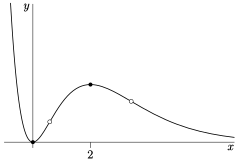
\includegraphics{graphE11}
%\end{center}
Open dots indicate inflection points, and closed dots indicate local extrema.
\begin{center}\begin{tikzpicture}[scale=1.2]
\YEaaxis{1}{6.2}{.25}{4}
\draw[thick] plot[domain=-.72:6, samples=100](\x,{3.7*\x*\x*exp(-\x)});
\draw (0,0) node[vertex]{};
\draw (2,2) node[vertex]{};
\draw (0.59,0.7) node[opendot]{};
\draw (3.4,1.4) node[opendot]{};
\YExcoord{2}{2}
\YExcoord{0.59}{2-\sqrt 2}
\YExcoord{3.4}{2+\sqrt 2}
\end{tikzpicture}\end{center}
\end{answer}
\begin{solution}
The parts of the question are just scaffolding to lead you through sketching the curve. Their answers are given explicitly, in an organized manner, in the ``answers" section. In this solution, they are scattered throughout.
\begin{itemize}
\item Asymptotes:

Since the function has a derivative at every real number, the function is continuous for every real number, so it has no vertical asymptotes. In the problem statement, you are told $\ds\lim_{x \to \infty} f(x)=0$, so $y=0$ is a horizontal asymptote as $x$ goes to infinity.  It remains to evaluate $\ds\lim_{x \to -\infty} f(x)$. Let's consider the limit of $f'(x)$ instead. Recall $K$ is a positive constant.
\begin{align*}
&\lim_{x \to -\infty}e^{-x}=\lim_{x \to \infty}e^x=\infty\\
&\lim_{x \to -\infty}K(2x-x^2)=-\infty
\intertext{So,}
&\lim_{x \to -\infty} K(2x-x^2)e^{-x}=-\infty
\end{align*}
That is, as $x$ becomes a hugely negative number, $f'(x)$ also becomes a hugely negative number. As we move left along the $x$-axis, $f(x)$ is decreasing with a steeper and steeper slope, as in the sketch below. That means
$\ds\lim_{x \to -\infty}f(x)=\infty$.
\begin{center}\begin{tikzpicture}
\YEaaxis{6}{1}{1}{8}
\draw[thick] (-1,1)--(-2,2) (-2.5,2.5)--(-3.5,4.5) (-3.75,5)--(-4.5,8);
\draw (-1.5,1.5) node[vertex]{};
\draw (-3,3.5) node[vertex]{};
\draw (-4.125,6.5) node[vertex]{};
\draw (-3,-1.5) node{Sketch: various tangent lines to $f(x)$,};
\draw (-3,-2) node{their slopes getting more strongly negative};
\draw (-3,-2.5) node{as $x$ gets more strongly negative.};
\end{tikzpicture}\end{center}
\item Intervals of increase and decrease:

We are given $f'(x)$ (although we don't know $f(x)$):
\[f'(x)=Kx(2-x)e^{-x}\]
The critical points of $f(x)$ are $x=0$ and $x=2$, and there are no singular points. Recall $e^{-x}$ is always positive, and $K$ is a positive constant.
\begin{center}\begin{tabular}{|c||c|c|c|c|c|}
\hline
$x$&$(-\infty,0)$&0&$(0,2)$&2&$(2,\infty)$\\
\hline
$f'(x)$&negative&0&positive&0&negative\\
\hline
$f(x)$& decreasing & local min & increasing & local max & decreasing\\
\hline
\end{tabular}\end{center}
So, $f(0)=0$ is a local minimum, and $f(2)=2$ is a local maximum.

Looking ahead to part \eqref{s3.6K4}, we have a skeleton of the curve.

\begin{center}\begin{tikzpicture}
\YEaaxis{4}{5.2}{.75}{4}
\draw[thick] (-4,4)--(0,0)--(2,2)--(4,.5)--(5,.25);
\draw (0,0) node[vertex]{};
\draw (2,2) node[vertex]{};
\draw[blue, decorate, decoration={brace, amplitude=10pt, mirror}] (-4,-1)--(0,-1);
\draw[blue] (-2,-1.75) node{decreasing};
\draw[red, decorate, decoration={brace, amplitude=10pt, mirror}] (0,-1)--(2,-1);
\draw[red] (1,-1.75) node{increasing};
\draw[blue, decorate, decoration={brace, amplitude=10pt, mirror}] (2,-1)--(4,-1);
\draw[blue] (3,-1.75) node{decreasing};
\YExcoord{2}{2}
\end{tikzpicture}\end{center}

\item Concavity:

Since we're given $f'(x)$, we can find $f''(x)$.
\begin{align*}
f''(x)&=K(2-2x-2x+x^2)e^{-x}\\
&=K(2-4x+x^2)e^{-x}\\
&=K\big(x-2-\sqrt{2}\big)\big(x-2+\sqrt{2}\big)e^{-x}
\end{align*}
where the last line can be found using the quadratic equation. So,
$f''(x)=0$  for $x=2\pm\sqrt{2}$, and $f''(x)$ exists everywhere.

\begin{center}\begin{tabular}{|c||c|c|c|c|c|}
\hline
$x$&$(-\infty,2-\sqrt{2})$&$2-\sqrt{2}$&$(2-\sqrt{2},2+\sqrt{2})$&$2+\sqrt 2$&$(2+\sqrt 2,\infty)$\\
\hline
$f'(x)$&positive&0&negative&0&positive\\
\hline
$f(x)$& concave up & IP & concave down & IP & concave up\\
\hline
\end{tabular}\end{center}

Now, we can add concavity to our sketch.

\begin{center}\begin{tikzpicture}[scale=1.2]
\YEaaxis{1}{6.2}{.25}{4}
\draw[thick] plot[domain=-.72:6, samples=100](\x,{3.7*\x*\x*exp(-\x)});
\draw (0,0) node[vertex]{};
\draw (2,2) node[vertex]{};
\draw (0.59,0.7) node[opendot]{};
\draw (3.4,1.4) node[opendot]{};
\YExcoord{2}{2}
\YExcoord{0.59}{2-\sqrt 2}
\YExcoord{3.4}{2+\sqrt 2}
\draw[blue, decorate, decoration={brace, amplitude=8pt, mirror}] (-1,-1)--(0,-1);
\draw[blue] (-.5,-1.5) node{decr};
\draw[red, decorate, decoration={brace, amplitude=10pt, mirror}] (0,-1)--(2,-1);
\draw[red] (1,-1.5) node{increasing};
\draw[blue, decorate, decoration={brace, amplitude=10pt, mirror}] (2,-1)--(6,-1);
\draw[blue] (4,-1.5) node{decreasing};
\draw[red, decorate, decoration={brace, amplitude=10pt, mirror}] (-1,-2.25)--(.59,-2.25);
\draw[red] (-.2,-2.75) node{cc up};
\draw[blue, decorate, decoration={brace, amplitude=10pt, mirror}] (.59,-2.25)--(3.4,-2.25);
\draw[blue] (2,-2.75) node{concave down};
\draw[red, decorate, decoration={brace, amplitude=10pt, mirror}] (3.4,-2.25)--(6,-2.25);
\draw[red] (4.7,-2.75) node{concave up};
\end{tikzpicture}\end{center}
%\begin{center}
%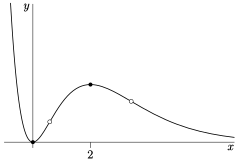
\includegraphics{graphE11}
%\end{center}
\end{itemize}
\end{solution}

\begin{question}[2010H]
 Let $f(x) = e^{-x}$ , $x \ge 0$.
\begin{enumerate}[(a)]
\item\label{s3.62010exp1} Sketch the graph of the equation $y = f(x)$. Indicate any
local extrema and inflection points.
\item\label{s3.62010exp4} Sketch the graph of  the inverse function $y = g (x)=f^{-1}(x)$.
\item\label{s3.62010exp2} Find the domain and range of the inverse function $g(x)= f^{-1}(x)$.
\item\label{s3.62010exp3} Evaluate $g'(\half)$.
\end{enumerate}
\end{question}
\begin{hint}
Once you have the graph of a function, reflect it over the line $y=x$ to graph its inverse.
Be careful of the fact that $f(x)$ is only defined in this problem for $x \geq 0$.
\end{hint}
\begin{answer}
\eqref{s3.62010exp1}
\begin{center}\begin{tikzpicture}
\YEaaxis{2}{6}{1}{6}
\draw[thick] plot[domain=0:5.5, samples=100](\x,{exp(-\x)}) node[above]{$y=f(x)$};
\YEycoord{1}{1};
\YExcoord{1}{1};
\draw (0,1) node[vertex]{};
\end{tikzpicture}\end{center}
There are no inflection points or extrema, except the endpoint $(0,1)$.

\eqref{s3.62010exp4}

\begin{center}\begin{tikzpicture}
\YEaaxis{2}{6}{2}{6}
\draw[thick, blue] plot[domain=0:5.5, samples=100]({exp(-\x)},\x) ;
\draw[blue] (1,1)node[right]{$y=g(x)$};
\YEycoord{1}{1};
\YExcoord{1}{1};
\draw[blue](1,0) node[vertex]{};
\end{tikzpicture}\end{center}
There are no inflection points or extrema, except the endpoint $(1,0)$.

\eqref{s3.62010exp2}
The domain of $g$ is  $(0,1]$.
The range of $g$ is $[0,\infty)$.

\eqref{s3.62010exp3}
$g'(\half)=-2$
\end{answer}
\begin{solution}
\eqref{s3.62010exp1}
You should be familiar with the graph of $y=e^x$. You can
           construct the graph of $y=e^{-x}$ just by reflecting the graph
           of $y=e^x$ across the $y$--axis. To see why this is the case,
           imagine swapping each value of $x$ its negative: for example,
                      swapping the point at $x = -1$ with the point at $x = 1$, etc.
           Alternatively, you can graph $y=f(x)=e^{-x}$, $x\ge 0$,
           using the methods of this section: at $x=0$, $y=f(0)=1$;
           as $x$ increases, $y=f(x)=e^{-x}$ decreases, with no local
           extrema; and as $x\rightarrow+\infty$, $y=f(x)\rightarrow 0$.

There are no inflection points or extrema, except the endpoint $(0,1)$.

\begin{center}\begin{tikzpicture}
\YEaaxis{2}{6}{1}{6}
\draw[thick, red] plot[domain=0:5.5, samples=100](\x,{exp(-\x)}) node[above]{$y=f(x)$};
\YEycoord{1}{1};
\YExcoord{1}{1};
\draw[red] (0,1) node[vertex]{};
\end{tikzpicture}\end{center}

\eqref{s3.62010exp4}

Recall that, to graph the inverse of a function, we reflect the original function across the line $y=x$.

You should be familiar with the graph of $y=e^x$. You can
           construct the graph of $y=e^{-x}$ just by reflecting the graph
           of $y=e^x$ across the $y$--axis. To see why this is the case,
           imagine swapping each value of $x$ its negative: for example,
           swapping the point at $x = -1$ with the point at $x = 1$, etc.

           Alternatively, you can graph $y=f(x)=e^{-x}$, $x\ge 0$,
           using the methods of this section: at $x=0$, $y=f(0)=1$;
           as $x$ increases, $y=f(x)=e^{-x}$ decreases, with no local
           extrema; and as $x\rightarrow+\infty$, $y=f(x)\rightarrow 0$.


           To see why this is true, consider the following. Since $g(x)$
           is the inverse of $f(x)$, then, for any pair of numbers $x$ and
           $y$, we have
           \begin{equation*}
                  f(x) = y\text{ if and only  }g(y) = x
          \end{equation*}
           That is, $g$ is the function that swaps the input and output
           of $f$. Now the point $(x,y)$ lies on the graph of $f$
           if and only if $y=f(x)$. Similarly, the point $(X,Y)$ lies
           on the graph of $g$ if and only if $Y=g(X)$. Setting $Y=x$
           and $X=y$ we see that the point $(y,x)$ lies on the graph of
           $g$ if and only if $x=g(y)$, which in turn is the case
           if and only if $y=f(x)$. So
           \begin{equation*}
                 \text{$(y,x)$ is on the graph of $g$ if and only
                        if $(x,y)$ is on the graph of $f$.}
           \end{equation*}
           To get from the point $(x,y)$ to the point $(y,x)$ we have to
           exchange $x \leftrightarrow y$, which we can do by reflecting
           over the line $y=x$.  Thus we can construct the graph of $g$
           by reflecting the curve $y = f(x)$ over the line  $y = x$.


\begin{center}\begin{tikzpicture}
\YEaaxis{2}{6}{2}{6}
\draw[thick, dashed, red] plot[domain=0:5.5, samples=100](\x,{exp(-\x)}) node[above]{$y=f(x)$};
\draw[dashed] (-2,-2)--(6,6) node[right]{$y=x$};
\draw[thick, blue] plot[domain=0:5.5, samples=100]({exp(-\x)},\x) ;
\draw[blue] (0,5)node[right]{$y=g(x)$};
\YEycoord{1}{1};
\YExcoord{1}{1};
\draw[red] (0,1) node[vertex]{};
\draw[blue] (1,0) node[vertex]{};
\end{tikzpicture}\end{center}

\eqref{s3.62010exp2}
The domain of $g$ is the range of $f$, which is $(0,1]$.
The range of $g$ is the domain of $f$, which is $[0,\infty)$.

\eqref{s3.62010exp3}
Since $g$ and $f$ are inverses,
\begin{align*}
g(f(x))&=x
\intertext{Using the chain rule,}
g'(f(x))\cdot f'(x)&=1
\intertext{Since $f'(x)=-e^{-x}=-f(x)$:}
g'(f(x))\cdot f(x)&=-1
\intertext{We plug in $f(x)=\frac{1}{2}$.}
g'\left(\frac{1}{2}\right)\cdot \frac{1}{2}&=-1\\
g'\left(\frac{1}{2}\right)&=-2
\end{align*}
\end{solution}




\begin{question}[2011H]
\begin{enumerate}[(a)]
\item Sketch the graph of $y=f(x)=x^5-x$, indicating asymptotes,
local maxima and minima, inflection points, and where the
graph is concave up/concave down.

\item Consider the function $f(x)=x^5-x+k$, where $k$ is a constant,
$-\infty<k<\infty$. How many roots does the function have? (Your answer might
depend on the value of $k$.)
\end{enumerate}
\end{question}
\begin{hint}

\end{hint}
\begin{answer}
(a)
\begin{center}\begin{tikzpicture}
\YEaxis{4}{4}
\draw[thick] plot[domain=-1.3:1.3, yscale=1.5, xscale=3, samples=100](\x,{\x*\x*\x*\x*\x-\x});
\draw (-2,.2) --(-2,-.2)node[below]{$\frac{-1}{\sqrt[4]{5}}$};
\draw (2,-.2) --(2,.2)node[above]{$\frac{1}{\sqrt[4]{5}}$};
\draw (.2,.78)--(-.2,.78) node[left]{$\frac{4}{5\sqrt[4]{5}}$};
\draw (.2,-.78)--(-.2,-.78) node[left]{$\frac{-4}{5\sqrt[4]{5}}$};
\end{tikzpicture}\end{center}
Local extrema are shown; inflection point at the origin.

(b) The number of distinct real roots of $x^5-x+k$ is:
\begin{itemize}
\item 1 when $|k|>\dfrac{4}{5\root{4}\of{5}}$
\item 2 when $|k|=\dfrac{4}{5\root{4}\of{5}}$
\item 3 when $|k|<\dfrac{4}{5\root{4}\of{5}}$
\end{itemize}
\end{answer}
\begin{solution}
(a)
First, we differentiate.
\[
f(x) = x^5-x\qquad
f'(x)=5x^4-1\qquad
f''(x)=20x^3\qquad
\]
The function and its first derivative tells us the following:
\begin{itemize}
\item $\ds\lim_{x \to \infty} f(x)=\infty$, $\ds\lim_{x \to -\infty} f(x)=-\infty$
\item $f'(x)> 0$ (i.e. $f$ is increasing) for
   $|x|> \dfrac{1}{\root{4}\of{5}}$
\item{}$f'(x)=0$ (i.e. $f$ has critical points) for $x= \pm\dfrac{1}{\root{4}\of{5}} \approx \pm 0.67$
\item{}$f'(x)< 0$ (i.e. $f$ is decreasing) for $|x| < \dfrac{1}{\root{4}\of{5}}$
\item $f\left(\pm\dfrac{1}{\sqrt[4]{5}}\right)=\mp\dfrac{4}{5\sqrt[4]{5}}\approx\mp0.53$
\end{itemize}
This gives us a first idea of the shape of the graph.
\begin{center}\begin{tikzpicture}
\YEaxis{5}{3}
\draw[->, thick] (-5,-3)--(-2,1.5);
\draw[->, thick] (-2,1.5)--(2,-1.5);
\draw[->, thick] (2,-1.5)--(5,3);
\draw (-2,.2) --(-2,-.2)node[below]{$\frac{-1}{\sqrt[4]{5}}$};
\draw (2,.2) --(2,-.2)node[below]{$\frac{1}{\sqrt[4]{5}}$};
\draw (.2,1.5)--(-.2,1.5) node[left]{$\frac{4}{5\sqrt[4]{5}}$};
\draw (.2,-1.5)--(-.2,-1.5) node[left]{$\frac{-4}{5\sqrt[4]{5}}$};
\end{tikzpicture}\end{center}
We refine this skeleton using information from the second derivative.
\begin{itemize}
\item $f''(x)> 0$ (i.e. $f$ is concave up) for $x> 0$,
%\hskip0.7in\smash{\figplace{OE11D_4}{0 in}{-0.3 in}}
\item{}$f''(x)=0$ (i.e. $f$ has an inflection point) for $x=0$, and
\item{}$f''(x)< 0$ (i.e. $f$ is concave down) for $x<0$
\end{itemize}
Thus
\begin{itemize}
\item $f$ has no asymptotes
\item $f$ has a local maximum at $x=-\dfrac{1}{\root{4}\of{5}}$
           and  a local minimum at $x=\dfrac{1}{\root{4}\of{5}}$
\item $f$ has an inflection point at $x=0$
\item $f$ is concave down for $x<0$ and concave up for $x>0$
\end{itemize}

\begin{center}\begin{tikzpicture}
\YEaxis{4}{4}
\draw[thick] plot[domain=-1.3:1.3, yscale=1.5, xscale=3, samples=100](\x,{\x*\x*\x*\x*\x-\x});
\draw (-2,.2) --(-2,-.2)node[below]{$\frac{-1}{\sqrt[4]{5}}$};
\draw (2,-.2) --(2,.2)node[above]{$\frac{1}{\sqrt[4]{5}}$};
\draw (.2,.78)--(-.2,.78) node[left]{$\frac{4}{5\sqrt[4]{5}}$};
\draw (.2,-.78)--(-.2,-.78) node[left]{$\frac{-4}{5\sqrt[4]{5}}$};
\end{tikzpicture}\end{center}
\medskip
(b) The function
$x^5-x+k$ has a root at $x=x_0$ if and only if $x^5-x=-k$
  at $x=x_0$. So the number of distinct real roots of $x^5-x+k$ is the
  number of times the curve $y=x^5-x$ crosses the horizontal line $y=-k$.
  The local maximum of $x^5-x$ (when $x=-\dfrac{1}{\root{4}\of{5}}$)
  is $\dfrac{4}{5\root{4}\of{5}}$, and the local minimum of $x^5-x$
 (when $x=\dfrac{1}{\root{4}\of{5}}$) is $-\dfrac{4}{5\root{4}\of{5}}$.
  So, looking at the graph of $x^5-x$ above, we see that the number of distinct
  real roots of $x^5-x+k$ is
\begin{itemize}
\item 1 when $|k|>\dfrac{4}{5\root{4}\of{5}}$
\item 2 when $|k|=\dfrac{4}{5\root{4}\of{5}}$
\item 3 when $|k|<\dfrac{4}{5\root{4}\of{5}}$
\end{itemize}
\end{solution}



\begin{question}[2012H]
The hyperbolic trigonometric functions $\sinh(x)$ and
$\cosh(x)$ are defined by
$$
\sinh(x)=\dfrac{e^x-e^{-x}}{2}\qquad
\cosh(x)=\dfrac{e^x+e^{-x}}{2}
$$
They have many properties that are similar to corresponding properties
of $\sin(x)$ and $\cos(x)$. In particular, it is easy to see that
$$
\diff{}{x} \sinh(x)=\cosh(x)\qquad
\diff{}{x} \cosh(x)=\sinh(x)\qquad
\cosh^2(x)-\sinh^2(x)=1
$$
You may use these properties in your solution to this question.
\begin{enumerate}[(a)]
\item Sketch the graphs of $\sinh(x)$ and $\cosh(x)$.
\item Define inverse hyperbolic trigonometric functions
$\sinh^{-1}(x)$ and $\cosh^{-1}(x)$, carefully specifying their domains
of definition. Sketch the graphs of $\sinh^{-1}(x)$ and $\cosh^{-1}(x)$.
\item Find
$
\dfrac{d\hfill}{dx}\left\{ \cosh^{-1}(x)\right\}
$.
\end{enumerate}
\end{question}
\begin{hint}
For (a), don't be intimidated by the new names: we can graph these functions using the methods learned in this section.

For (b), remember that to define an inverse of a function, we need to restrict the domain of that function to an interval where it is one-to-one. Then to graph the inverse, we can simply reflect the original function over the line $y=x$.

For (c), set $y(x)=\cosh^{-1}(x)$, so $\cosh(y(x))=x$. The differentiate using the chain rule. To get your final answer in terms of $x$ (instead of $y$), use the identity $\cosh^2(y)-\sinh^2(y)=1$.
\end{hint}
\begin{answer}
(a)
\begin{center}
\begin{tikzpicture}
\YEaxis{3}{3}
\draw plot[domain=-3:3, scale=0.3](\x,{sinh(\x)});
\draw (2,3) node[right]{$y=\sinh x$};
\end{tikzpicture}
\begin{tikzpicture}
\YEaaxis{3}{3}{.5}{3}
\draw plot[domain=-3:3, scale=0.3](\x,{cosh(\x)});
\draw (2,3) node[right]{$y=\cosh x$};
\draw (.2,.3)--(-.4,.3) node[left]{1};
\draw (0,-3) node{};
\end{tikzpicture}\end{center}

(b)
For any real $x$, define $\sinh^{-1}(x)$ to be
the unique solution of $\sinh(y)=x$. For every $x\in[1,\infty)$, define $\cosh^{-1}(x)$ to be the
unique $y\in[0,\infty)$ that obeys $\cosh(y)=x$.

\begin{center}
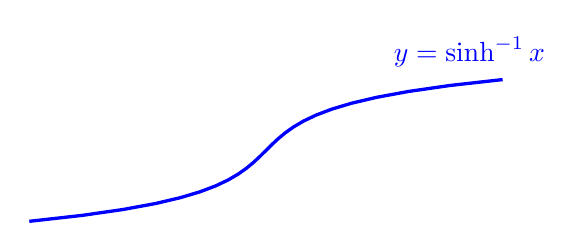
\begin{tikzpicture}
\YEaxis{3}{2}
\draw[blue, very thick] plot[domain=-3:3, scale=0.3]({sinh(\x)},\x);
\draw[blue] (1.5,1.25) node[right]{$y=\sinh^{-1} x$};
\end{tikzpicture}\hfill
\begin{tikzpicture}
\YEaaxis{3}{3}{.5}{2}
\draw[blue, very thick] plot[domain=0:3, scale=0.3]({cosh(\x)},\x);
\draw[blue] (1.5,1.25) node[right]{$y=\cosh^{-1} x$};
\draw (0,-2) node{};
\end{tikzpicture}
\end{center}

(c) $\ds\diff{}{x}\{\cosh^{-1}(x)\}=\dfrac{1}{\sqrt{x^2-1}}$
\end{answer}
\begin{solution}

 (a)
 You might not be familiar with hyperbolic sine and cosine, but you don't need to be. We can graph them using  the same methods as the other curves in this section. The derivatives are given to us:
 \[\diff{}{x}\{\sinh x\}=\cosh x =\frac{e^x+e^{-x}}{2}\qquad\diff{}{x}\{\cosh x\}=\sinh x = \frac{e^x-e^{-x}}{2}\]
 \[\left(\diff{}{x}\right)^2\{\sinh x\}=\sinh x =\frac{e^x-e^{-x}}{2}\qquad
 \left(\diff{}{x}\right)^2\{\cosh x\}=\cosh x = \frac{e^x+e^{-x}}{2}\]
  Observe that:
 \begin{itemize}
 \item $\sinh(x)$ has a derivative that is always positive, so $\sinh(x)$ is always increasing. The second derivative of $\sinh(x)$ is negative to the left of $x=0$ and positive to the right of $x=0$, so $\sinh(x)$ is concave down to the left of the $y$-axis and concave up to its right, with an inflection point at $x=0$.
  \item $\cosh(x)$ has a derivative that is positive when $x>0$ and negative when $x<0$. The second derivative of $\cosh(x)$ is always positive, so it is always concave up.
\item $\cosh(0)=1$ and $\sinh(0)=0$.
\item
 $\ds\lim_{x\rightarrow\infty}\sinh x = \ds\lim_{x\rightarrow\infty}\cosh x
 =\ds\lim_{x\rightarrow\infty}\frac{e^x}{2}=\infty$, since $\ds\lim_{x \to \infty}e^{-x}=0$
\item
$\ds\lim_{x \to -\infty}\sinh x =\ds\lim_{x \to -\infty}\left(\frac{e^x}{2}-\frac{e^{-x}}{2}\right)
=\ds\lim_{x \to \infty}\left(\frac{e^{-x}}{2}-\frac{e^x}{2}\right)=-\infty
$ and\\
$\ds\lim_{x \to -\infty}\cosh x =\ds\lim_{x \to -\infty}\left(\frac{e^x}{2}+\frac{e^{-x}}{2}\right)
=\ds\lim_{x \to \infty}\left(\frac{e^{-x}}{2}+\frac{e^x}{2}\right)=\infty
$
\item $\cosh(x)$ is even, since $\cosh(-x)=\dfrac{e^{-x}+e^{-(-x)}}{2}=\dfrac{e^{-x}+e^x}{2}=\cosh (x)$, and\\
$\sinh (x)$ is odd, since $\sinh(-x)=\dfrac{e^{-x}-e^{-(-x)}}{2}=\dfrac{e^{-x}-e^x}{2}=\dfrac{-\left(e^x-e^{-x}\right)}{2}=-\sinh(x)$
\end{itemize}

\begin{center}
\begin{tikzpicture}
\YEaxis{3}{3}
\draw plot[domain=-3:3, scale=0.3](\x,{sinh(\x)});
\draw (2,3) node[right]{$y=\sinh x$};
\end{tikzpicture}
\begin{tikzpicture}
\YEaaxis{3}{3}{.5}{3}
\draw plot[domain=-3:3, scale=0.3](\x,{cosh(\x)});
\draw (2,3) node[right]{$y=\cosh x$};
\draw (.2,.3)--(-.4,.3) node[left]{1};
\draw (0,-3) node{};
\end{tikzpicture}\end{center}


(b)
\begin{itemize}\item As $y$ runs over $(-\infty,\infty)$ the function
$\sinh(y)$ takes every real value exactly once. So,
for each $x\in(-\infty,\infty)$, define $\sinh^{-1}(x)$ to be
the unique solution of $\sinh(y)=x$.
\item As $y$ runs over $[0,\infty)$ the function
$\cosh(y)$ takes every real value in $[1,\infty)$ exactly once.
In particular, the smallest value of $\cosh(y)$ is $\cosh(0)=1$.
So, for each $x\in[1,\infty)$, define $\cosh^{-1}(x)$ to be the
unique $y\in[0,\infty)$ that obeys $\cosh(y)=x$.
\end{itemize} To graph the inverse of a (one-to-one) function, we reflect the original function over the line $y=x$. Using this method to graph $y=\sinh^{-1}(x)$ is straightforward. To graph $y=\cosh(x)$, we need to be careful of the domains: we are restricting $\cosh(x)$ to values of $x$ in $[0,\infty)$.
The graphs are

\begin{center}
\begin{tikzpicture}
\YEaxis{3}{3}
\draw[red, thin] plot[domain=-3:3, scale=0.3](\x,{sinh(\x)});
\draw[red] (1,3) node[below right]{$y=\sinh x$};
\draw[dashed] (-3,-3)--(2,2);% node[right]{$y=x$};
\draw[blue, very thick] plot[domain=-3:3, scale=0.3]({sinh(\x)},\x);
\draw[blue] (1.5,1.25) node[right]{$y=\sinh^{-1} x$};
\draw[ultra thick, ->] (4,0)--(5,0);
\end{tikzpicture}
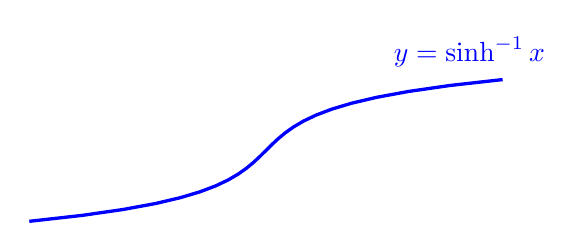
\begin{tikzpicture}
\YEaxis{3}{3}
\draw[blue, very thick] plot[domain=-3:3, scale=0.3]({sinh(\x)},\x);
\draw[blue] (1.5,1.25) node[right]{$y=\sinh^{-1} x$};
\end{tikzpicture}

\begin{tikzpicture}
\YEaaxis{3}{3}{.5}{2}
\draw[red, thin] plot[domain=0:3, scale=0.3](\x,{cosh(\x)});
\draw[red] (1,3) node[below right]{$y=\cosh x$};
\draw[dashed] (-1,-1)--(2,2);% node[right]{$y=x$};
\draw[blue, very thick] plot[domain=0:3, scale=0.3]({cosh(\x)},\x);
\draw[blue] (1.5,1.25) node[right]{$y=\cosh^{-1} x$};
\draw[ultra thick, ->] (4,1)--(5,1);
\end{tikzpicture}
\begin{tikzpicture}
\YEaaxis{3}{3}{.5}{2}
\draw[blue, very thick] plot[domain=0:3, scale=0.3]({cosh(\x)},\x);
\draw[blue] (1.5,1.25) node[right]{$y=\cosh^{-1} x$};
\draw (-1,-1) node{};
\end{tikzpicture}
\end{center}
%\centerline{\figput{graphE12A}\hskip1in\figplace{graphE12B}{0in}{0.5in}}

\item{}(c) Let $y(x)= \cosh^{-1}(x)$. Then, using the definition of $\cosh^{-1}$,
\begin{align*}
\cosh y(x)&=x
\intertext{We differentiate with respect to $x$ using the chain rule.}
\diff{}{x}\left\{\cosh y(x)\right\}&=\diff{}{x}\{x\}\\
y'(x) \sinh y(x)&=1
\intertext{We solve for $y'(x)$.}
y'(x) &=\dfrac{1}{\sinh y(x)}
\intertext{We want to have our answer in terms of $x$, not $y$. We know that $\cosh y=x$, so if we can convert hyperbolic sine into hyperbolic cosine, we can get rid of $y$. Our tool for this is the identity, given in the question statement, $\cosh^2(x)-\sinh^2(x)=1$. This tells us $\sinh^2(y)=1-\cosh^2(y)$.
Now we have to decide whether $\sinh(y)$ is the positive or negative square root of $1-\cosh^2(y)$ in our context. Looking at the graph of $y(x)=\cosh^{-1}(x)$, we see $y'(x)>0$. So we use the positive square root:}
y'(x) & =\dfrac{1}{\sqrt{\cosh^2 y(x)-1}}
  =\dfrac{1}{\sqrt{x^2-1}}
\end{align*}
Remark: $\ds\diff{}{x}\left\{\arccos(x)\right\}=\dfrac{-1}{\sqrt{1-x^2}}$, so again the hyperbolic trigonometric function has properties similar to (but not exactly the same as) its trigonometric counterpart.
\end{solution}
